%%%%%%%%%%%%%%%%%%%%%%%%%%%%%%%%%%%%%%%%%%%%%%%%%%%%%%%%%%%%%%%%%%%%%%%%%%%%%%%%%%%%%%%%
% Setup I6pd2 style, common packages
%%%%%%%%%%%%%%%%%%%%%%%%%%%%%%%%%%%%%%%%%%%%%%%%%%%%%%%%%%%%%%%%%%%%%%%%%%%%%%%%%%%%%%%%
\documentclass[final,hyperref={pdfpagelabels=false},noamsthm]{beamer}
\usepackage{default}

\usetheme{I6pd2} % Use the I6pd2 theme supplied with this template

\usepackage[english]{babel} % English language/hyphenation

\usepackage{amsmath,amsthm}
\usepackage{multirow}

\usepackage{tikz}
\usetikzlibrary{fit}					% fitting shapes to coordinates
\usetikzlibrary{backgrounds}	% drawing the background after the foreground

%%%%%%%%%%%%%%%%%%%%%%%%%%%%%%%%%%%%%%%%%%%%%%%%%%%%%%%%%%%%%%%%%%%%%%%%%%%%%%%%%%%%%%%%
% Shortcuts for this project
%%%%%%%%%%%%%%%%%%%%%%%%%%%%%%%%%%%%%%%%%%%%%%%%%%%%%%%%%%%%%%%%%%%%%%%%%%%%%%%%%%%%%%%%

% blackboard series
\def\bbP{\mathbb{P}}
\def\bbp{\mathbb{p}}
\def\bbE{\mathbb{E}}
\def\bbN{\mathbb{N}}

% calligraphic series
\def\calT{\mathcal{T}}
\def\calW{\mathcal{W}}
\def\calX{\mathcal{X}}

% bold series
\def\bfP{\mathbf{P}}
\def\bfX{\mathbf{X}}

% distributions
\def\aDist{\Lambda}
\def\aTime{T}
\def\Geom{\text{Geom}}

% stuff
\newcommand{\prob}{\mathbb{P}}
\newcommand{\calV}{\mathcal{V}}
\newcommand{\calE}{\mathcal{E}}
\newcommand{\ee}{Z} % ends of edges
\newcommand{\bfee}{\mathbf{\ee}}
\newcommand{\bfE}{\mathbf{E}}
\newcommand{\PYP}{\mathcal{PYP}}
\newcommand{\geom}{\beta}
\newcommand{\BNTL}{\text{\rm BNTL}}
\newcommand{\bfT}{\mathbf{T}}
\newcommand{\calO}{\mathcal{O}}
\newcommand{\bbR}{\mathbb{R}}
\newcommand{\bfPsi}{\boldsymbol{\Psi}}
\newcommand{\bfn}{\mathbf{n}}
\newcommand{\bfd}{\mathbf{d}}
\newcommand{\argdot}{{\,\vcenter{\hbox{\scalebox{0.5}{$\bullet$}}}\,}}%{\bullet}
\def\indicator{\mathbf{1}}
\newcommand{\limscale}[2]{\overset{\scriptscriptstyle{#1 \uparrow #2}}{\widesim[1.25]}}
\newcommand{\simiid}{\overset{\scriptscriptstyle{\text{i.i.d.}}}{\widesim}}
\newcommand{\widesim}[1][1.5]{
	\mathrel{\scalebox{#1}[1]{$\sim$}}
}

%%%%%%%%%%%%%%%%%%%%%%%%%%%%%%%%%%%%%%%%%%%%%%%%%%%%%%%%%%%%%%%%%%%%%%%%%%%%%%%%%%%%%%%%
% Define footer contents
%%%%%%%%%%%%%%%%%%%%%%%%%%%%%%%%%%%%%%%%%%%%%%%%%%%%%%%%%%%%%%%%%%%%%%%%%%%%%%%%%%%%%%%%

\newcommand{\leftfoot}{} % Left footer text

\newcommand{\rightfoot}{~ \url{http://csml.stats.ox.ac.uk/learning/}} % Right footer text


\title{Sampling and Inference for Beta Neutral-to-the-Left Models of Sparse Networks} % Poster title

\author{Benjamin Bloem-Reddy, \underline{Adam Foster}, Emile Mathieu, Yee Whye Teh }
\institute{Department of Statistics, University of Oxford}

%%%%%%%%%%%%%%%%%%%%%%%%%%%%%%%%%%%%%%%%%%%%%%%%%%%%%%%%%%%%%%%%%%%%%%%%%%%%%%%%%%%%%%%%
% Main presentation
%%%%%%%%%%%%%%%%%%%%%%%%%%%%%%%%%%%%%%%%%%%%%%%%%%%%%%%%%%%%%%%%%%%%%%%%%%%%%%%%%%%%%%%%

\begin{document}
	
\begin{frame}[plain]
	\titlepage
\end{frame}

\begin{frame}
	\frametitle{Contents}
	\tableofcontents
\end{frame}

\section{Background}

\begin{frame}
	\frametitle{Temporal networks}
	\textbf{Examples}
	\begin{itemize}
		\item Messages between people (email, WhatsApp, ...)
		\item Posts + replies on StackOverflow
	\end{itemize}
	
\end{frame}

\begin{frame}
	\frametitle{Temporal networks}
	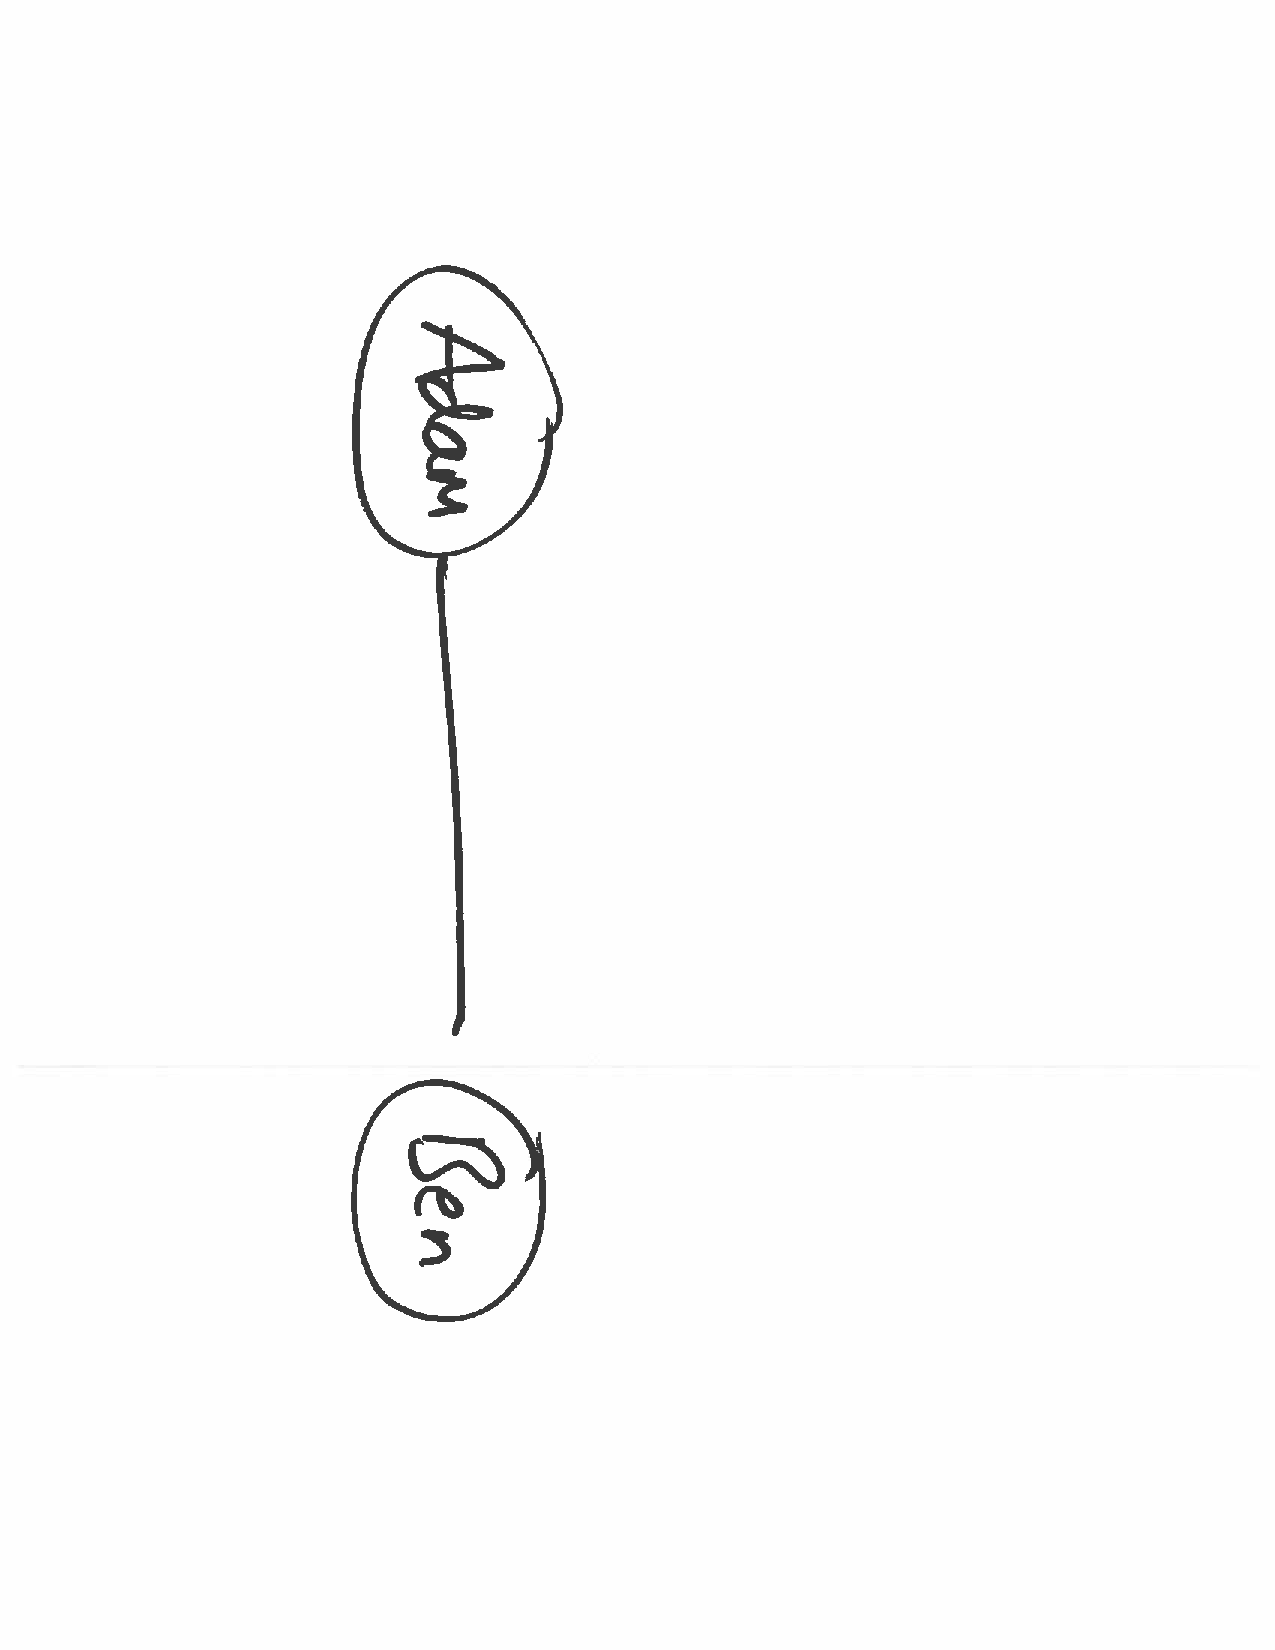
\includegraphics[angle=90,origin=c,scale=0.4]{fig/socialnet1}
\end{frame}

\begin{frame}
	\frametitle{Temporal networks}
	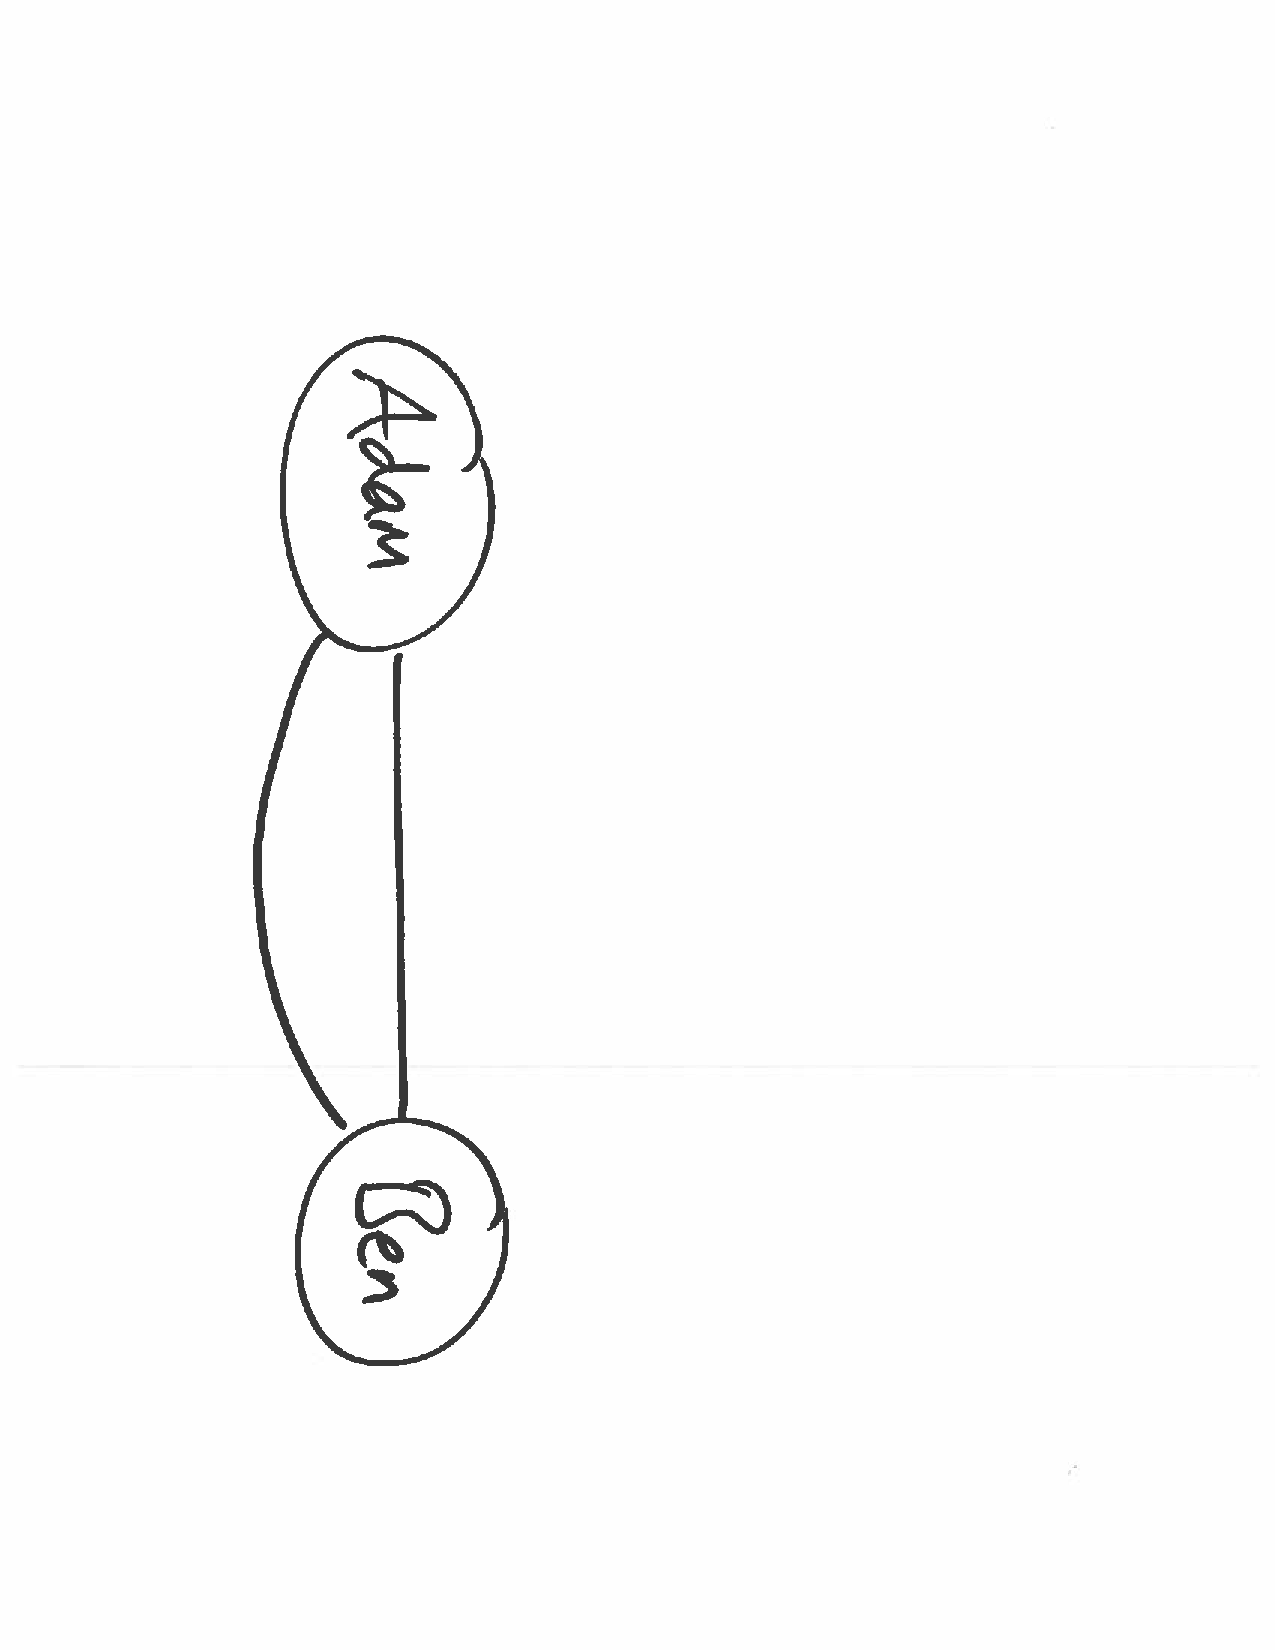
\includegraphics[angle=90,origin=c,scale=0.4]{fig/socialnet2}
\end{frame}

\begin{frame}
	\frametitle{Temporal networks}
	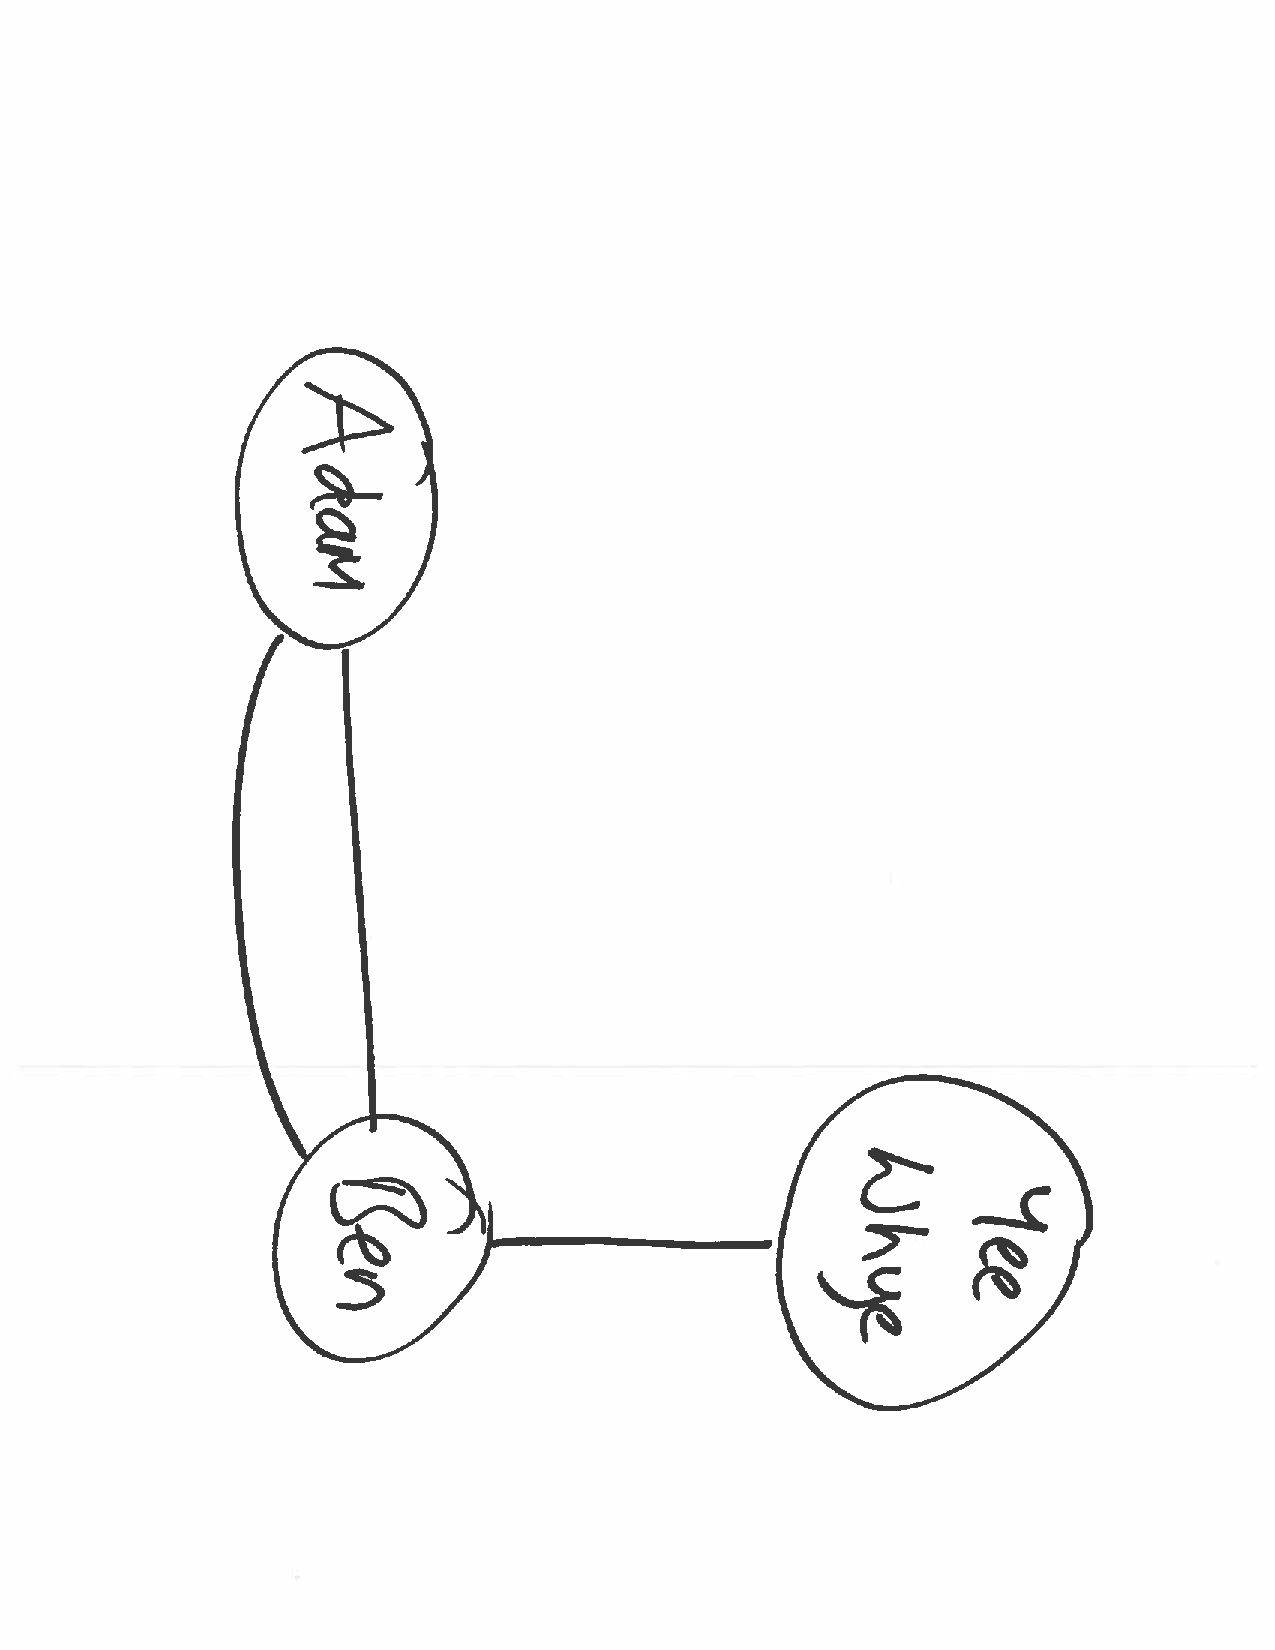
\includegraphics[angle=90,origin=c,scale=0.4]{fig/socialnet3}
\end{frame}

\begin{frame}
	\frametitle{Temporal networks}
	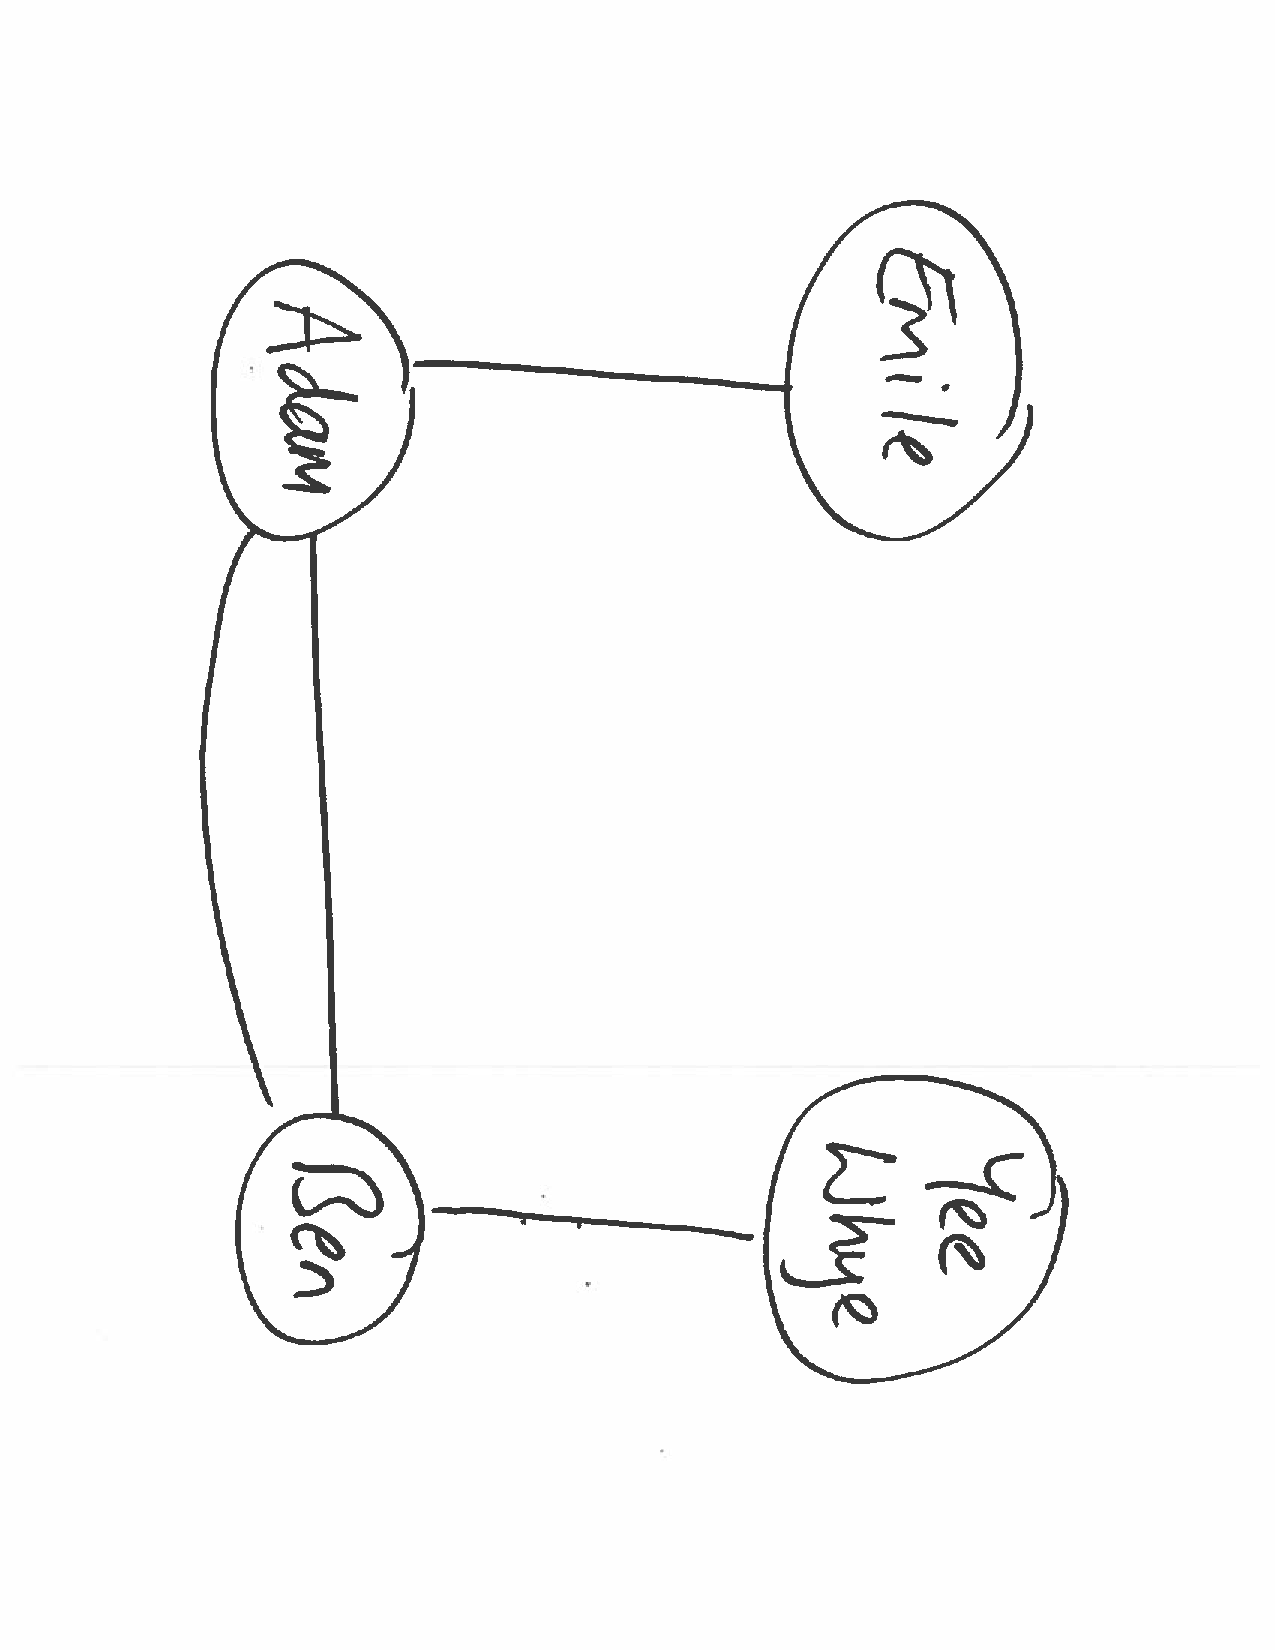
\includegraphics[angle=90,origin=c,scale=0.4]{fig/socialnet4}
\end{frame}


\begin{frame}
	\frametitle{Sparsity}
	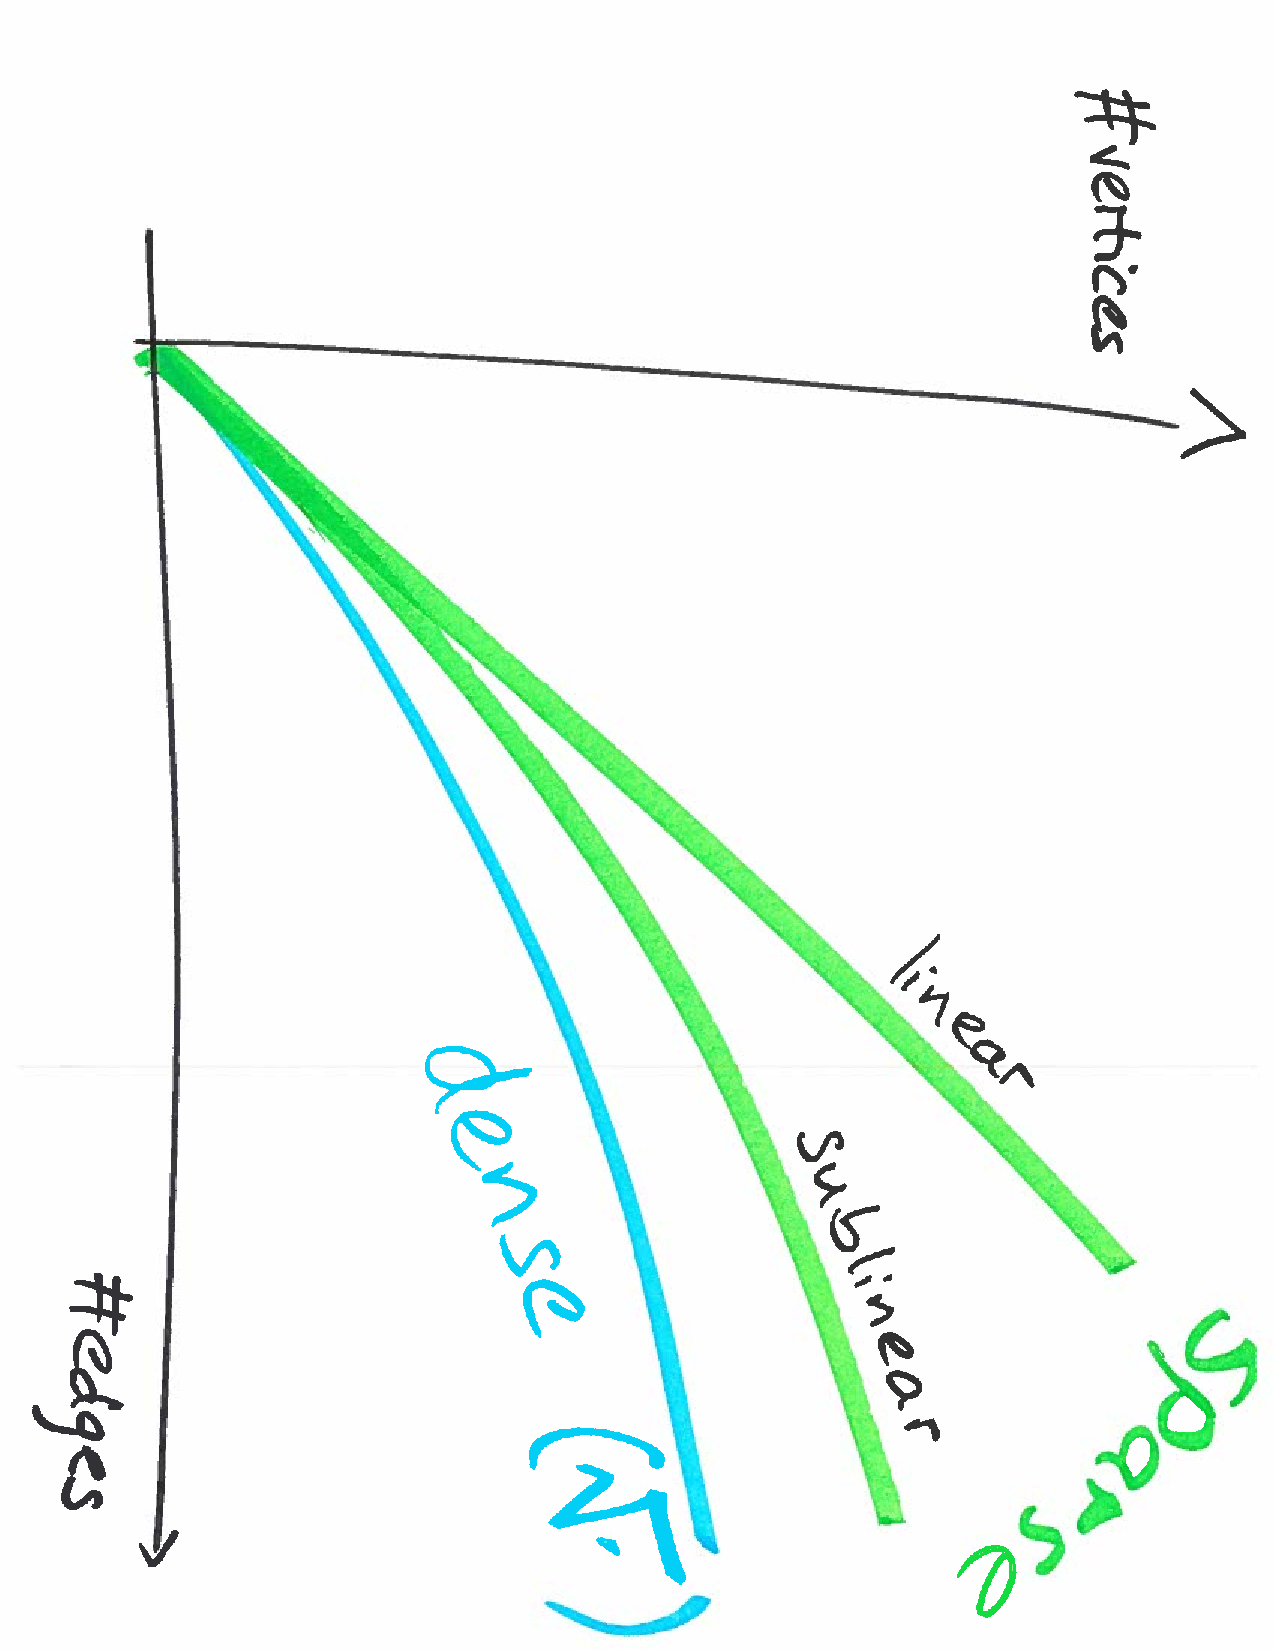
\includegraphics[angle=90,origin=c,scale=0.37]{fig/sparsity}
\end{frame}

\begin{frame}
	\frametitle{Power law degree distribution}
	Power law distribution of exponent $\eta$\
	\begin{equation*}
	p(d) \propto d^{-\eta} 
	\end{equation*}
	where $\eta > 1$
\end{frame}

\begin{frame}
	\frametitle{Power law degree distribution}
	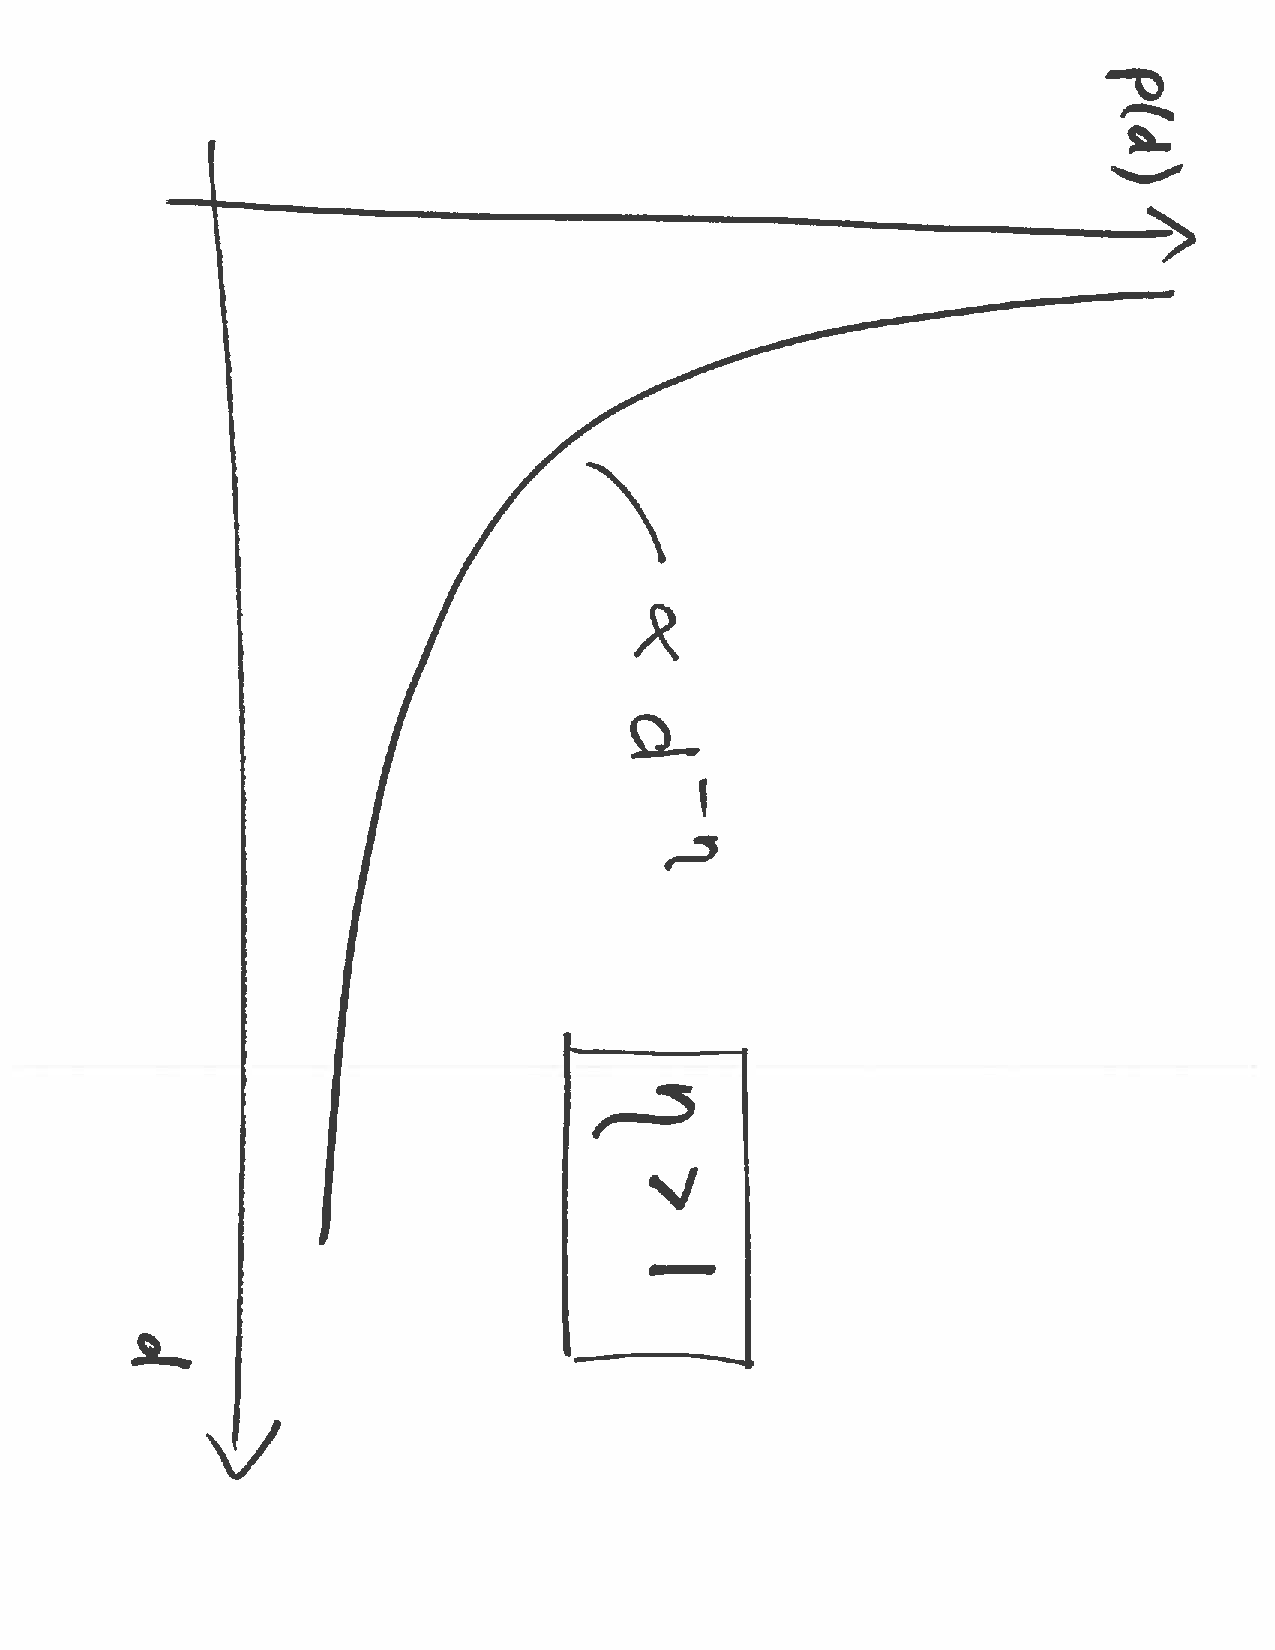
\includegraphics[angle=90,origin=c,scale=0.37]{fig/powerlaw}
\end{frame}

\begin{frame}
	\frametitle{Sparity and power law}
	\begin{align*}
	\textbf{Sublinear } \text{sparsity} & \quad \iff \quad  \eta \in (1,2) \\
	\textbf{Linear } \text{sparsity} & \quad \iff \quad \eta > 2
	\end{align*}
\end{frame}

\begin{frame}
	\frametitle{Empirical study}
	\textbf{SNAP datasets} \cite{snapnets}
	\begin{table}[b]
		% \vspace*{-\baselineskip}
		\label{tab:datasets}
		\begin{center}
			\begin{tabular}{lll}
				Dataset                 & \# of vertices   & \# of edges    \\
				\hline
				Ask Ubuntu    & 159,316   & 964,437    \\
				UCI social network   & 1,899     & 20,296     \\
				EU email        & 986       & 332,334    \\
				Math Overflow & 24,818    & 506,550    \\
				Stack Overflow           & 2,601,977 & 63,497,050 \\
				Super User    & 194,085   & 1,443,339  \\
				Wikipedia talk pages    & 1,140,149 & 7,833,140 \\
			\end{tabular}
		\end{center}
	\end{table}
	
\end{frame}

\begin{frame}
	\frametitle{Ask Ubuntu}
	\begin{figure}[h]
		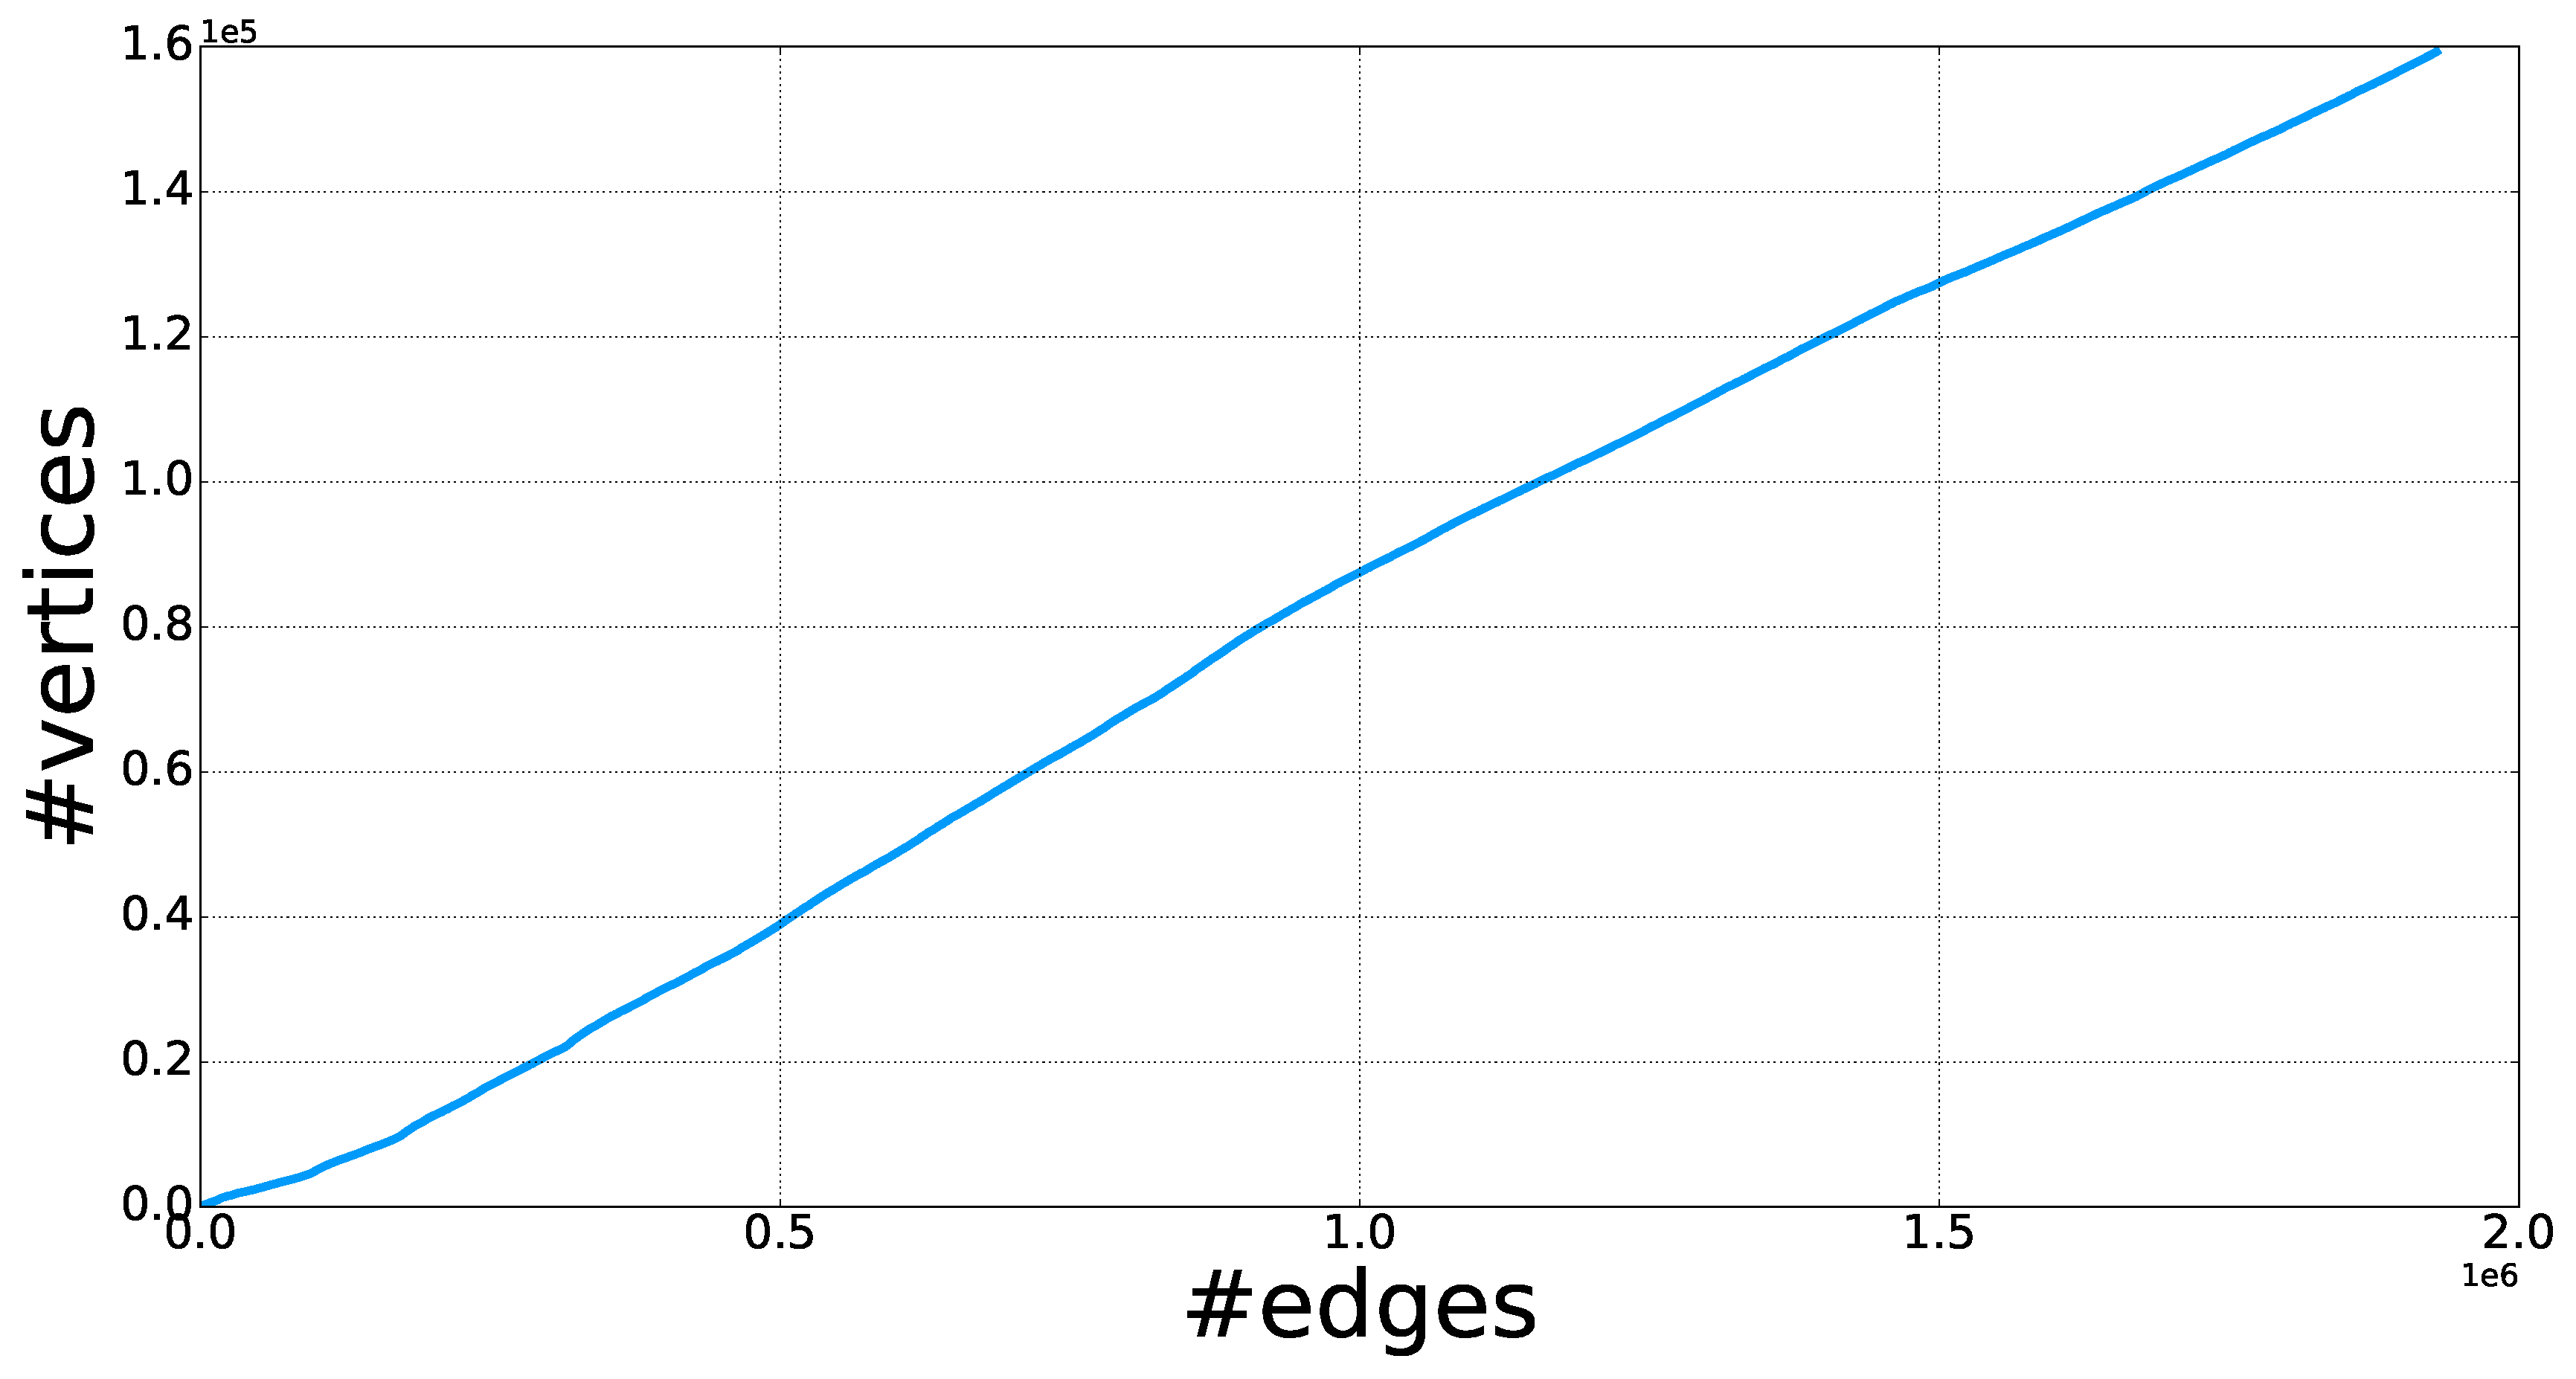
\includegraphics[width=1.0\textwidth]{fig/n_askubuntu_arrival.pdf}
	\end{figure}
	%$\hat{\sigma}=-0.0990787$
	%$\hat{\sigma} = -0.099$
\end{frame}

\begin{frame}
	\frametitle{UCI social network}
	\begin{figure}[h]
		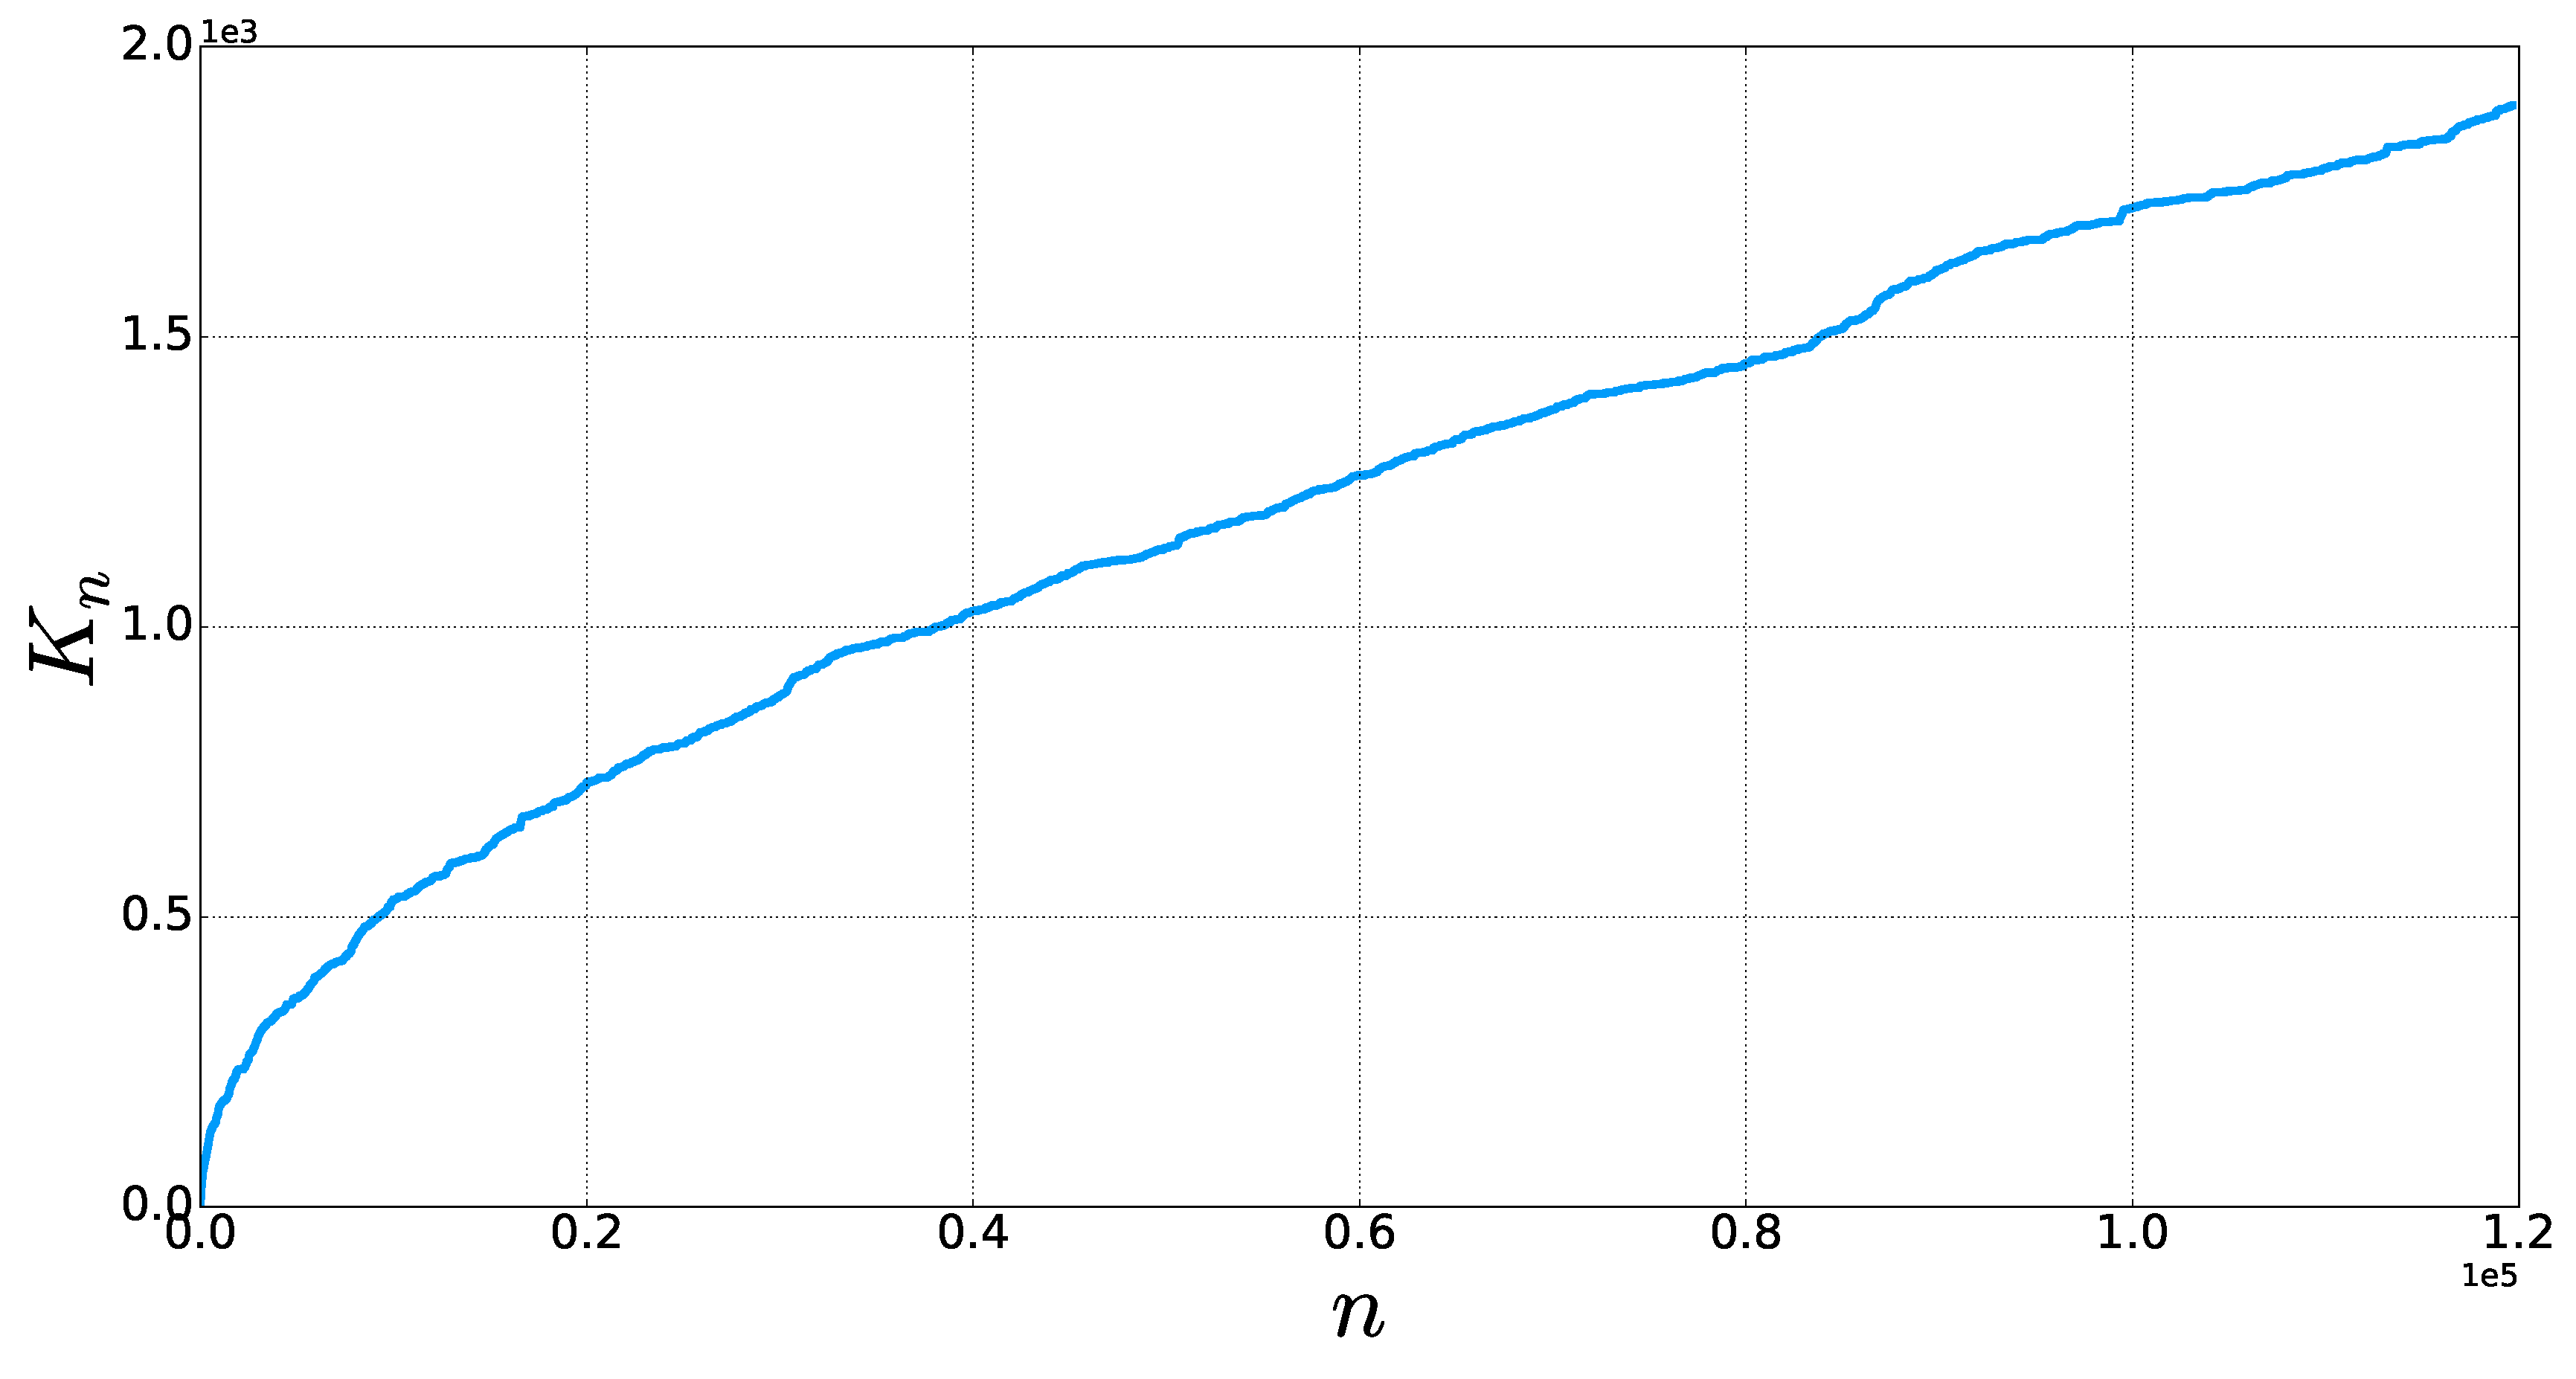
\includegraphics[width=1.0\textwidth]{fig/n_CollegeMsg_arrival.pdf}
	\end{figure}
	% $\sigma=0.95228934$
	% $\hat{\sigma} = 0.952$
\end{frame}

\begin{frame}
	\frametitle{Ask Ubuntu degree distribution}
	\begin{figure}[h]
		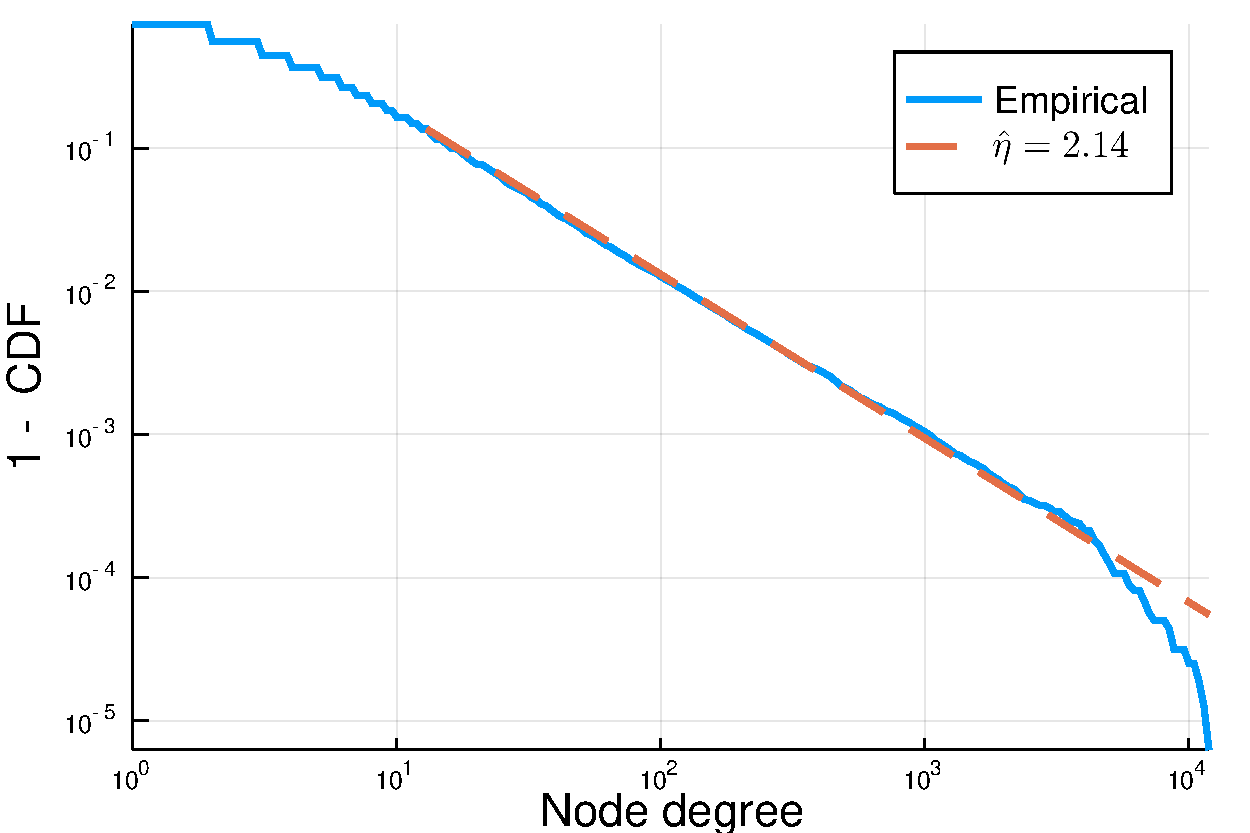
\includegraphics[width=0.8\textwidth]{fig/nodes_degre_power_law_askubuntu.pdf}
	\end{figure}
	
	$\hat{\eta} = 2.14$ estimated using technique of \cite{clauset}
	
\end{frame}


\begin{frame}
	\frametitle{Models}
	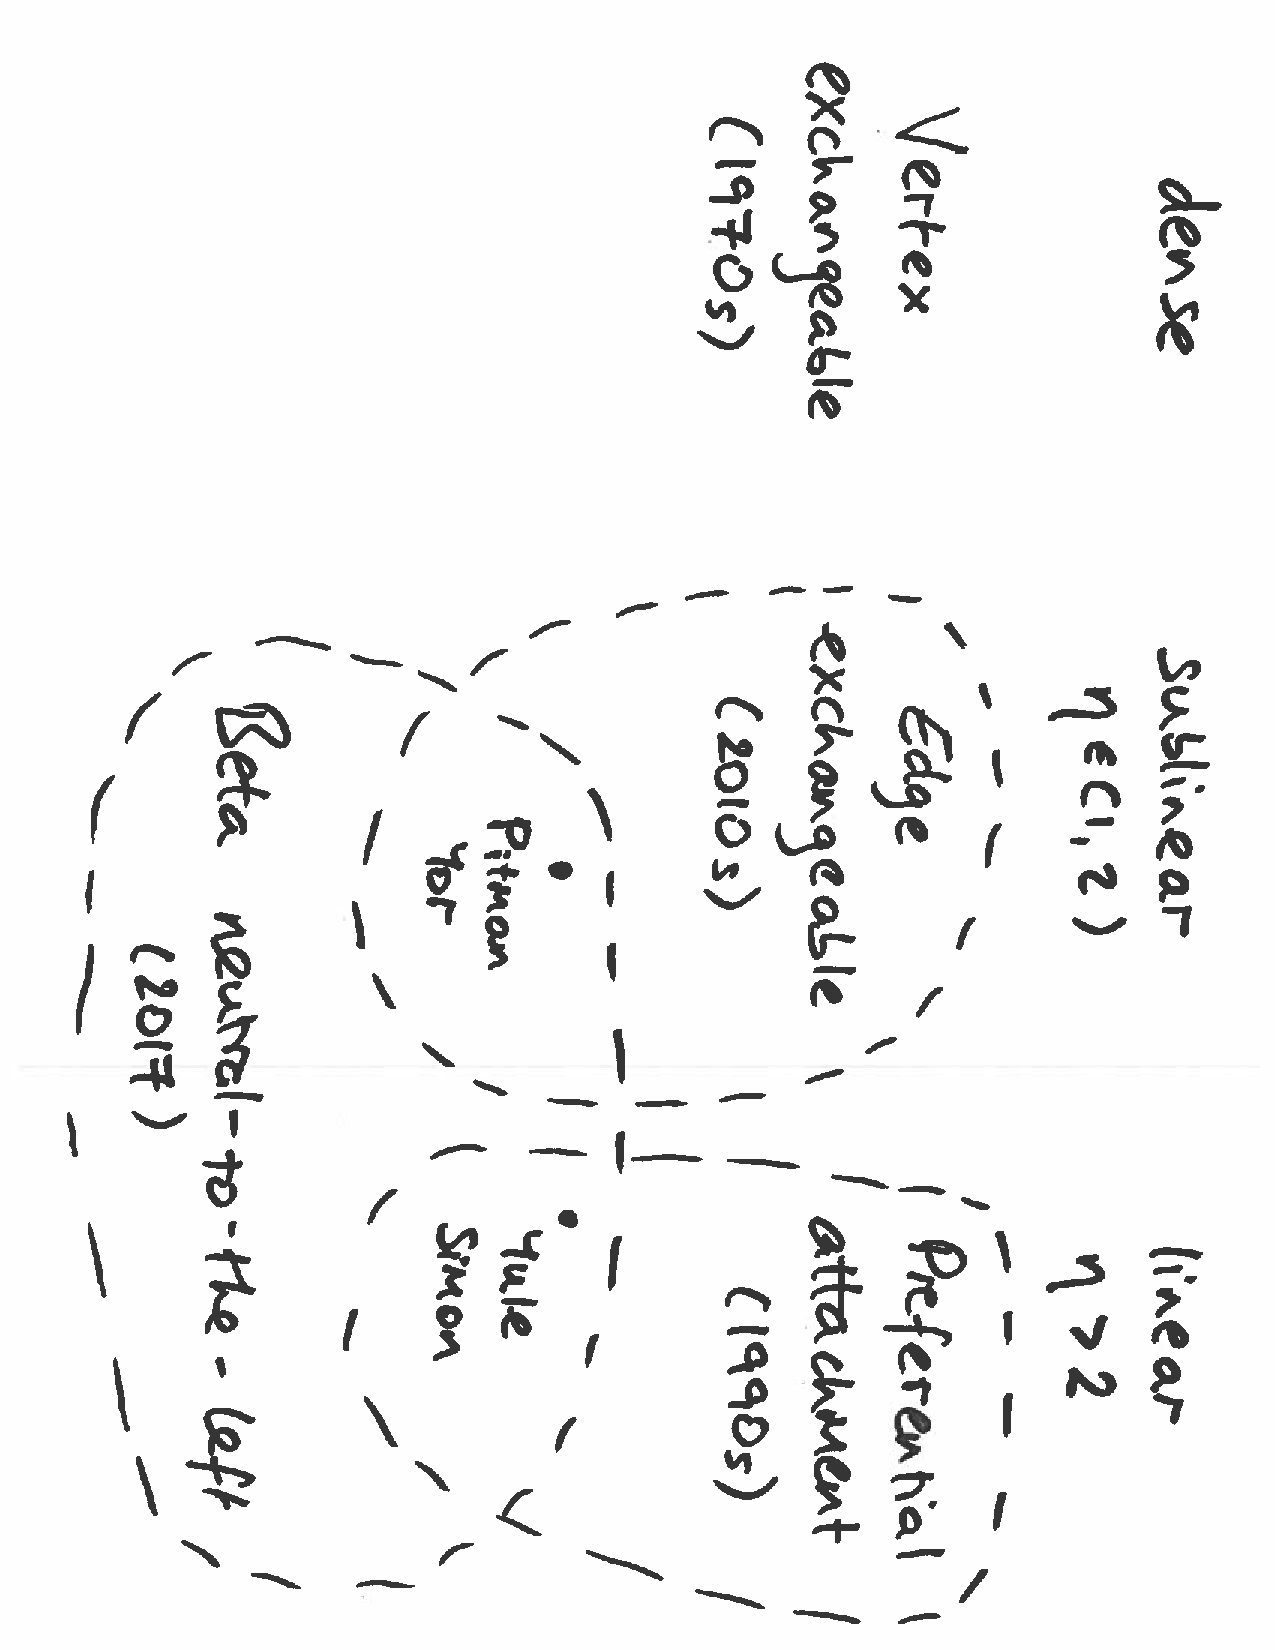
\includegraphics[angle=90,origin=c,scale=0.4]{fig/models}
\end{frame}

\begin{frame}
	\frametitle{Yule-Simon Process}
	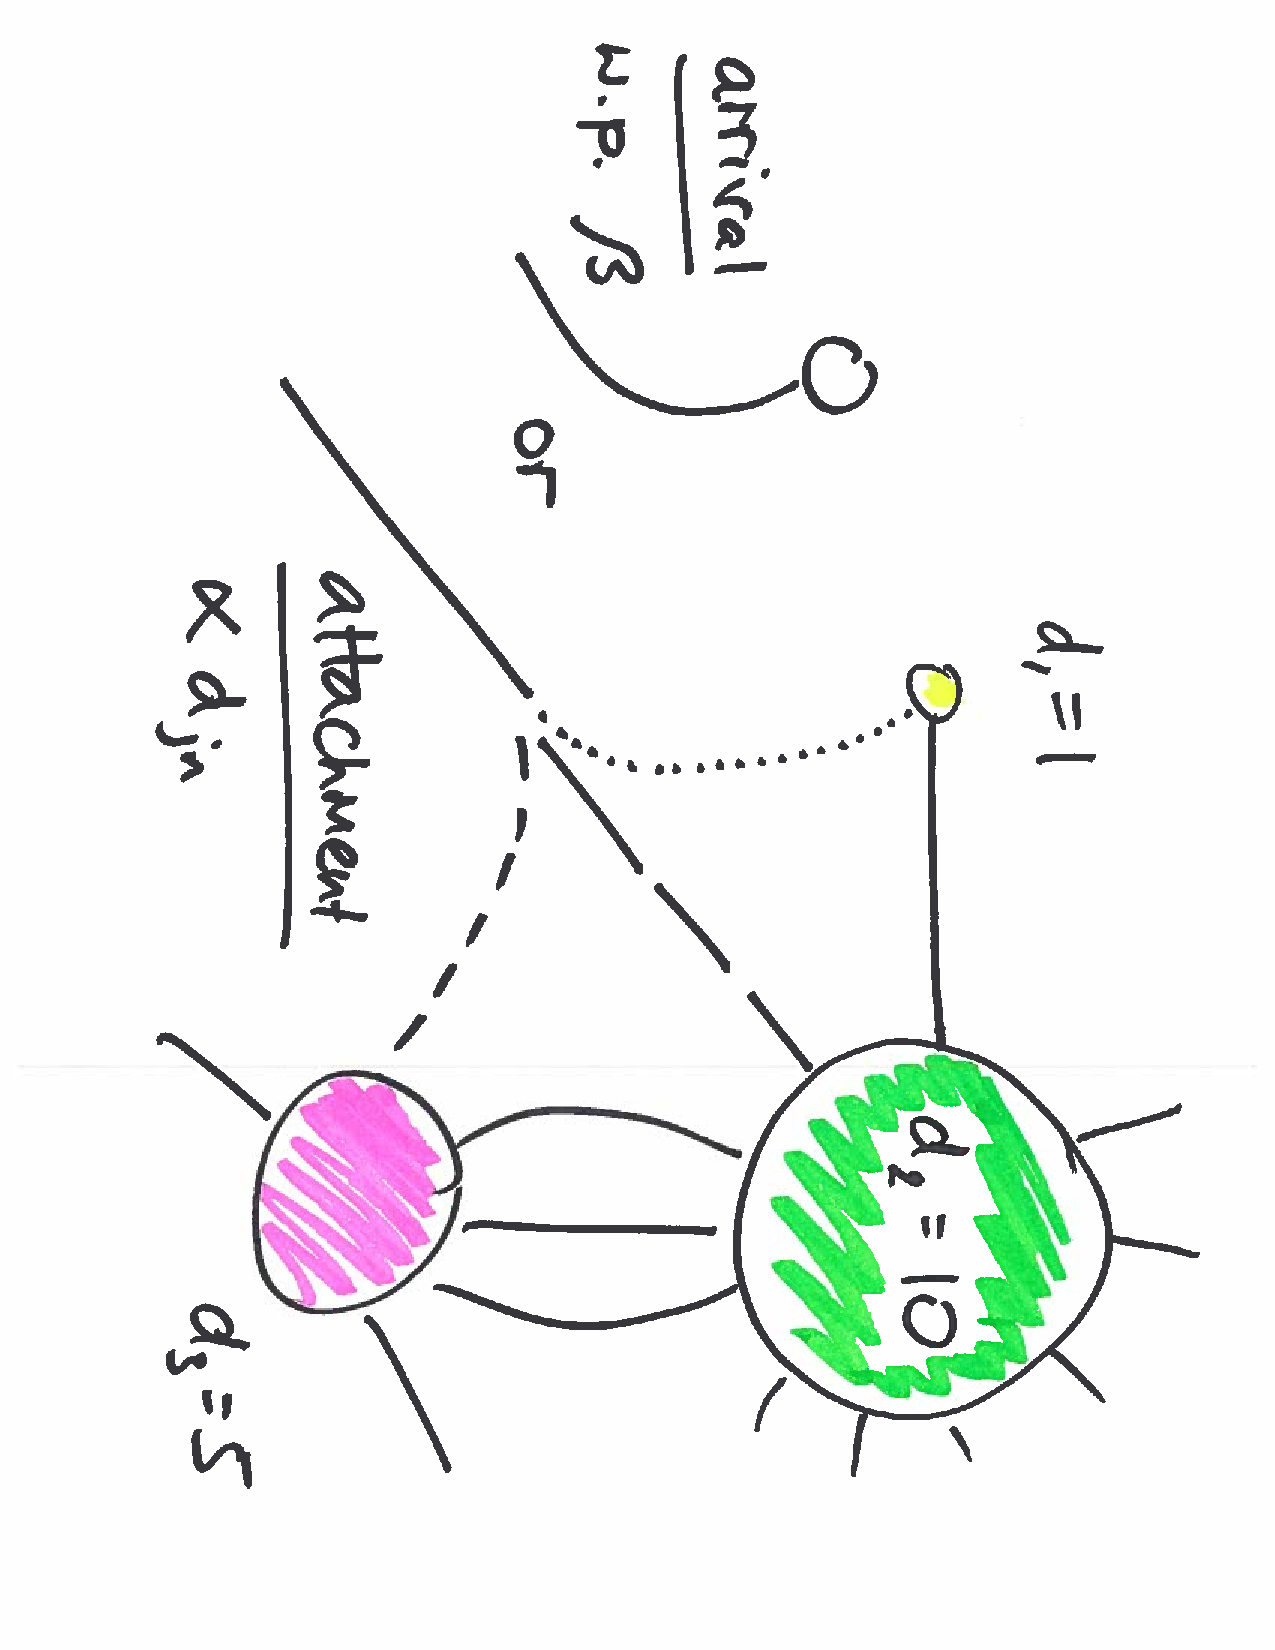
\includegraphics[angle=90,origin=c,scale=0.4]{fig/ys}
\end{frame}

\begin{frame}
	\frametitle{Yule-Simon Process}
	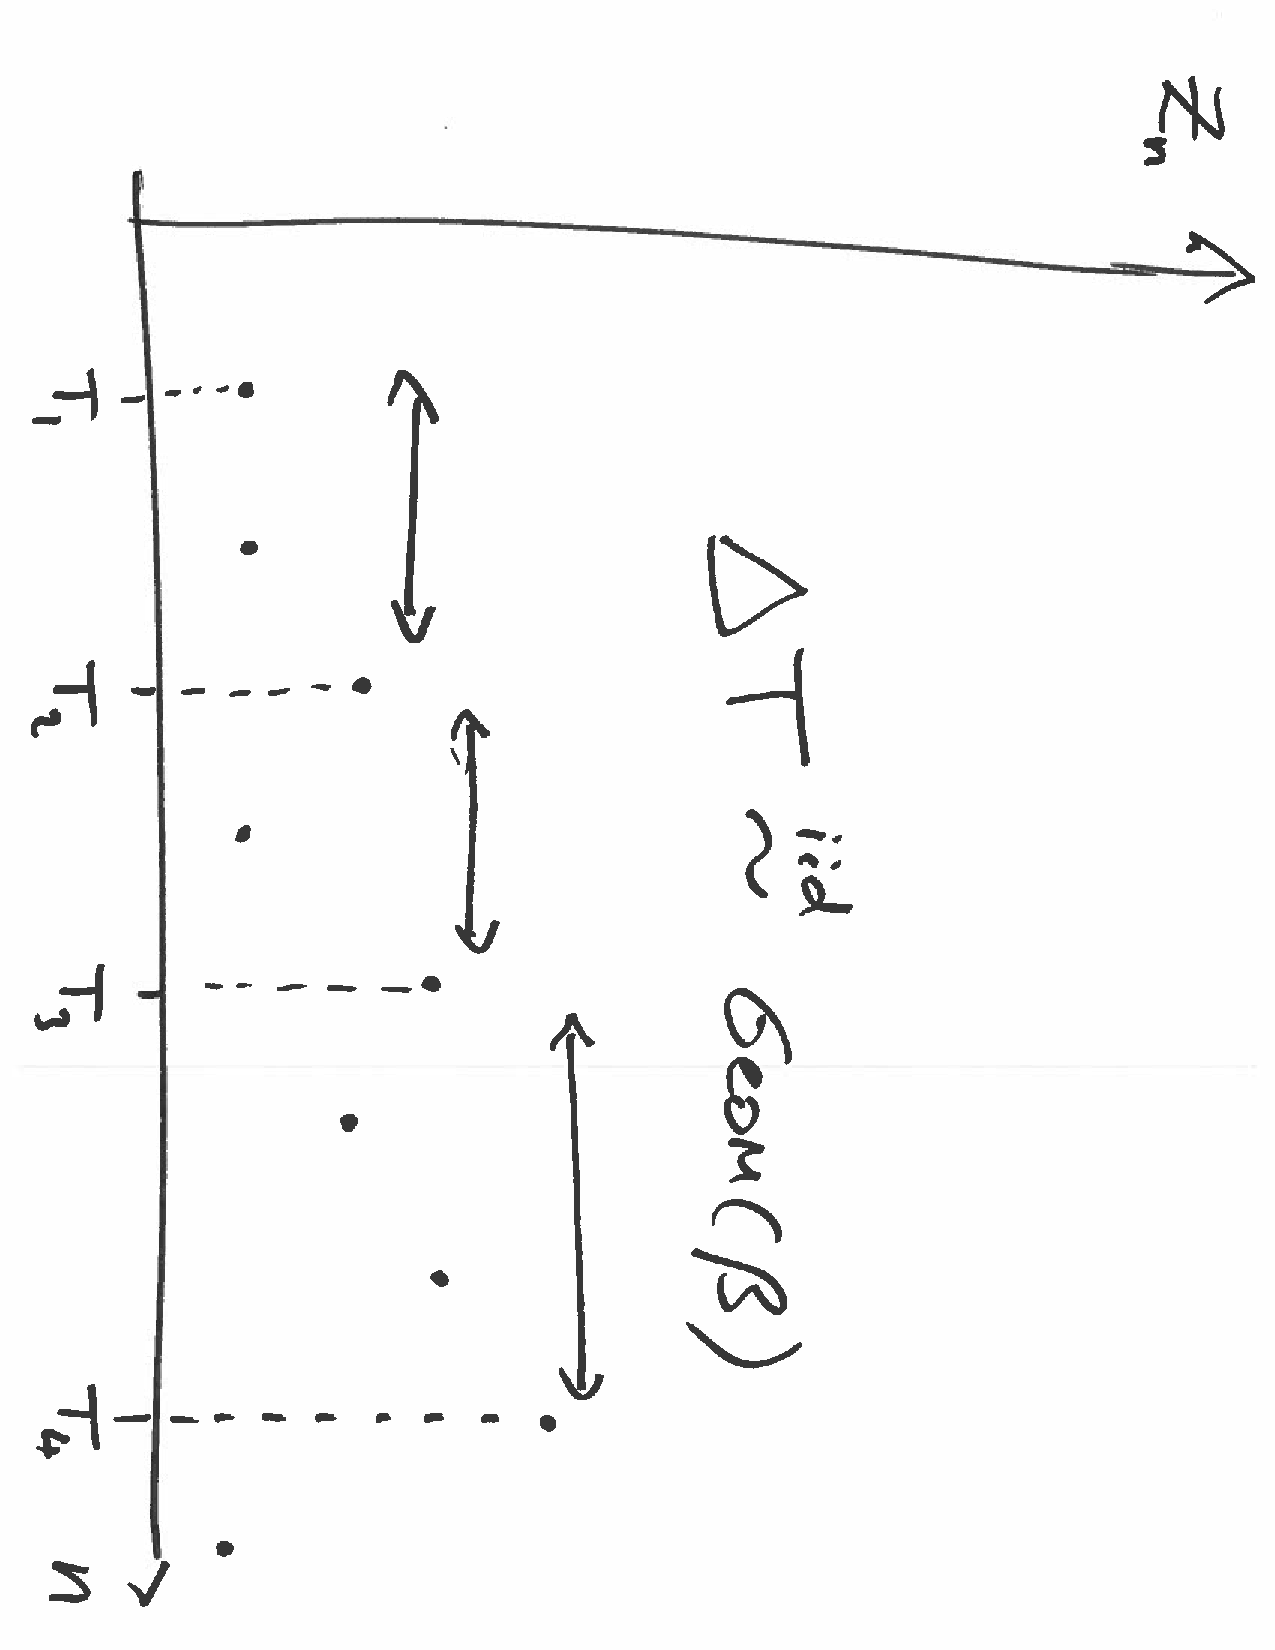
\includegraphics[angle=90,origin=c,scale=0.37]{fig/ys2}
\end{frame}

\begin{frame}
	\frametitle{Yule-Simon Process}
	Asymptotic power law degree distribution with
	\begin{equation*}
		\eta = 1 + \frac{1}{1-\beta} > 2
	\end{equation*}
\end{frame}

\begin{frame}
	\frametitle{Pitman-Yor Process}
	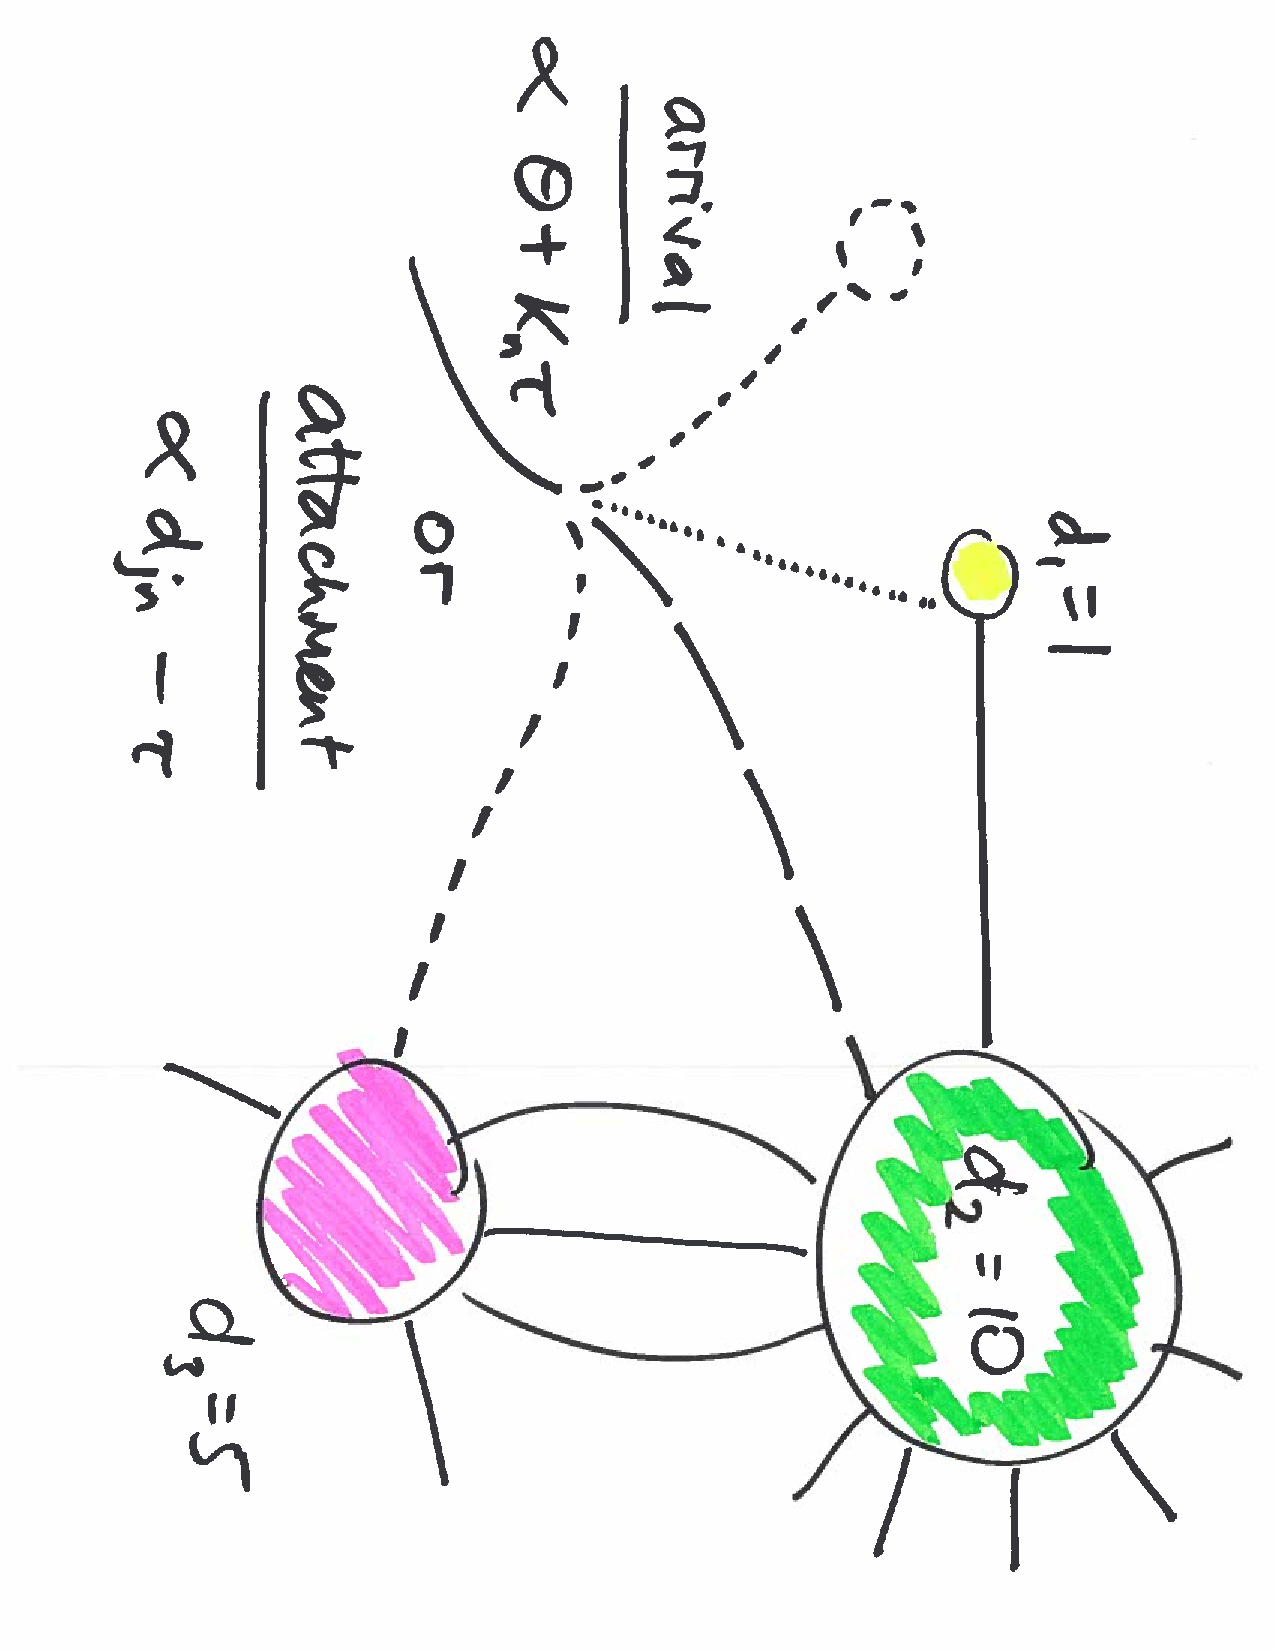
\includegraphics[angle=90,origin=c,scale=0.4]{fig/pyp}
\end{frame}

\begin{frame}
	\frametitle{Pitman-Yor Process}
	Asymptotic power law degree distribution with
	\begin{equation*}
		\eta = 1 + \tau \in (1, 2)
	\end{equation*}
	and $K_n = o(n)$
\end{frame}


\begin{frame}
	\frametitle{Edge exchangeable models \cite{cai2016}, \cite{CraneDempsey2017}}
	``The probability of all orderings of edge arrivals is the same''
	
	\vspace{20pt}
	\begin{itemize}
		\item Sublinear sparsity
		\item $\eta \in (1,2)$
	\end{itemize}
	
\end{frame}

\begin{frame}
	\frametitle{Beta Neutral-to-the-left Process \cite{Bloem2017}}
	\vspace{2pt}
	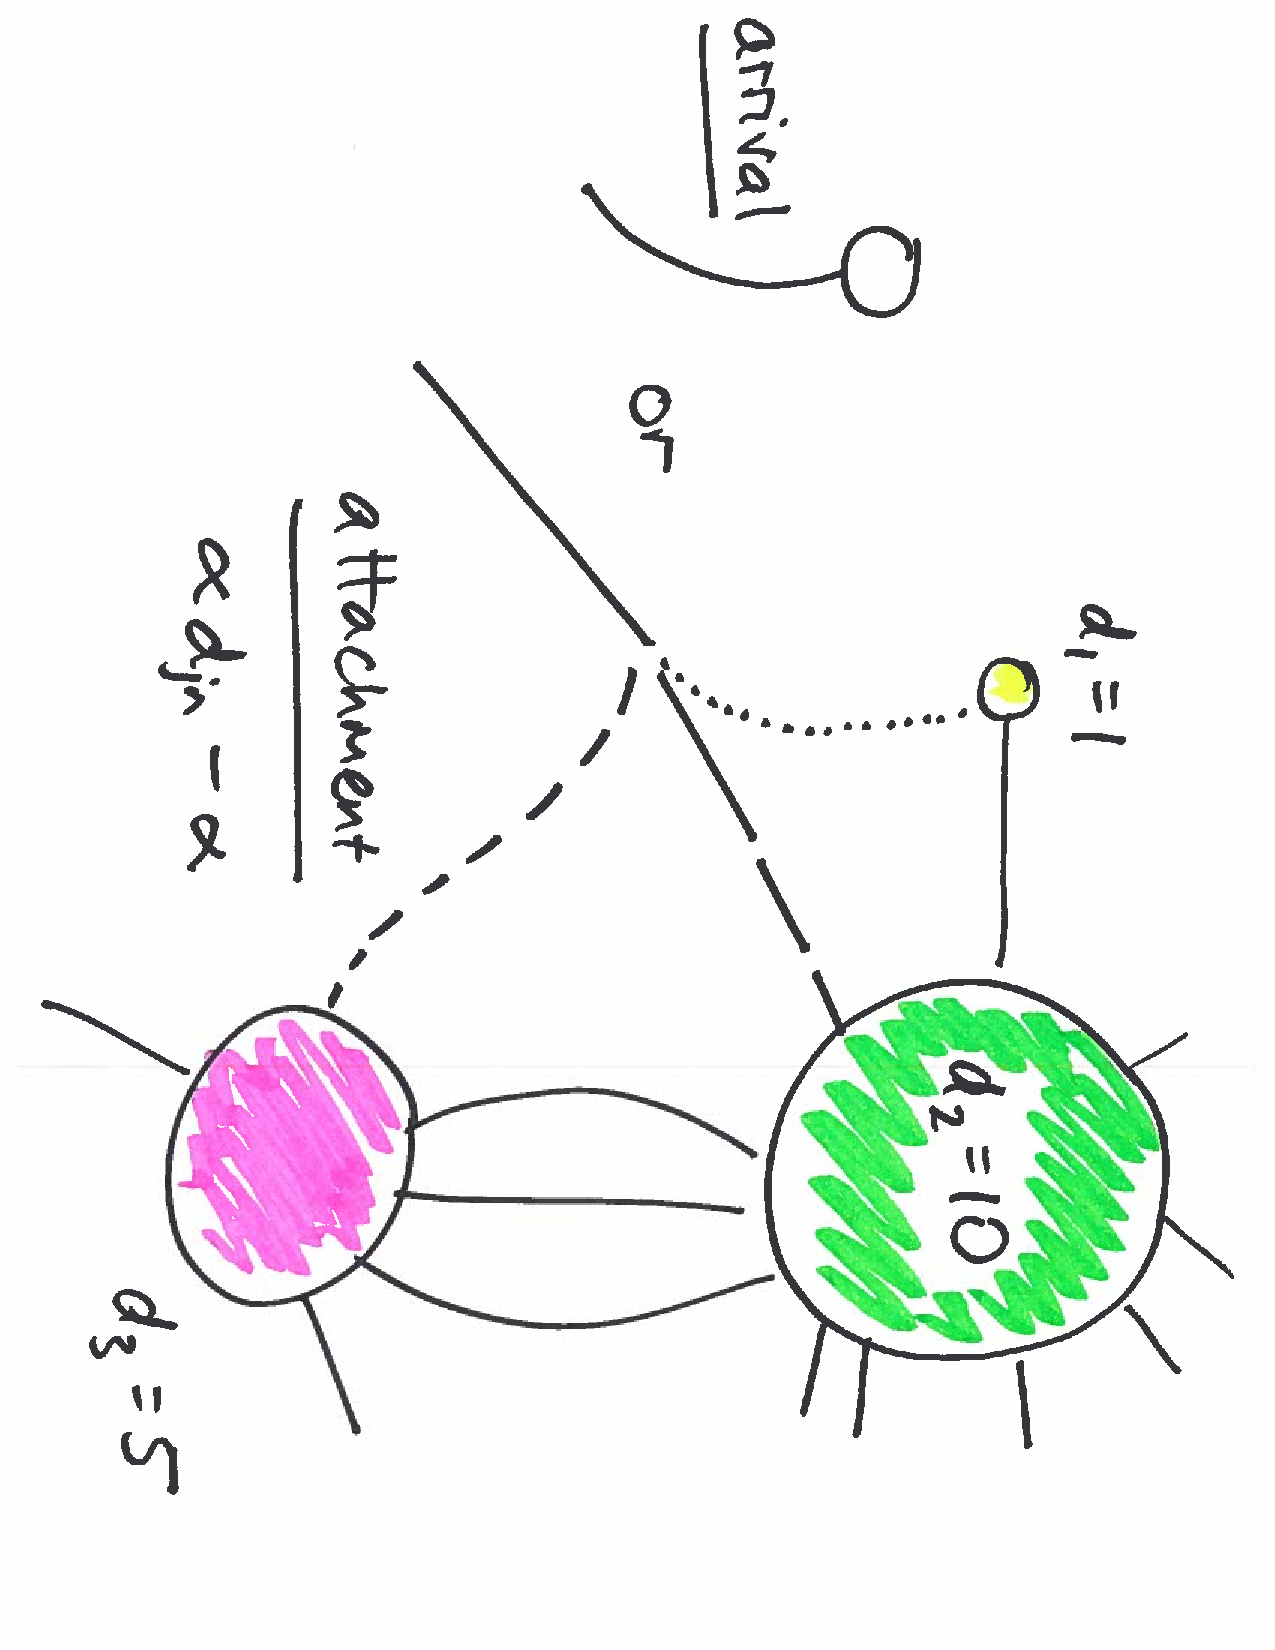
\includegraphics[angle=90,origin=c,scale=0.37]{fig/bntl}
\end{frame}

\begin{frame}
	\frametitle{Models -- again}
	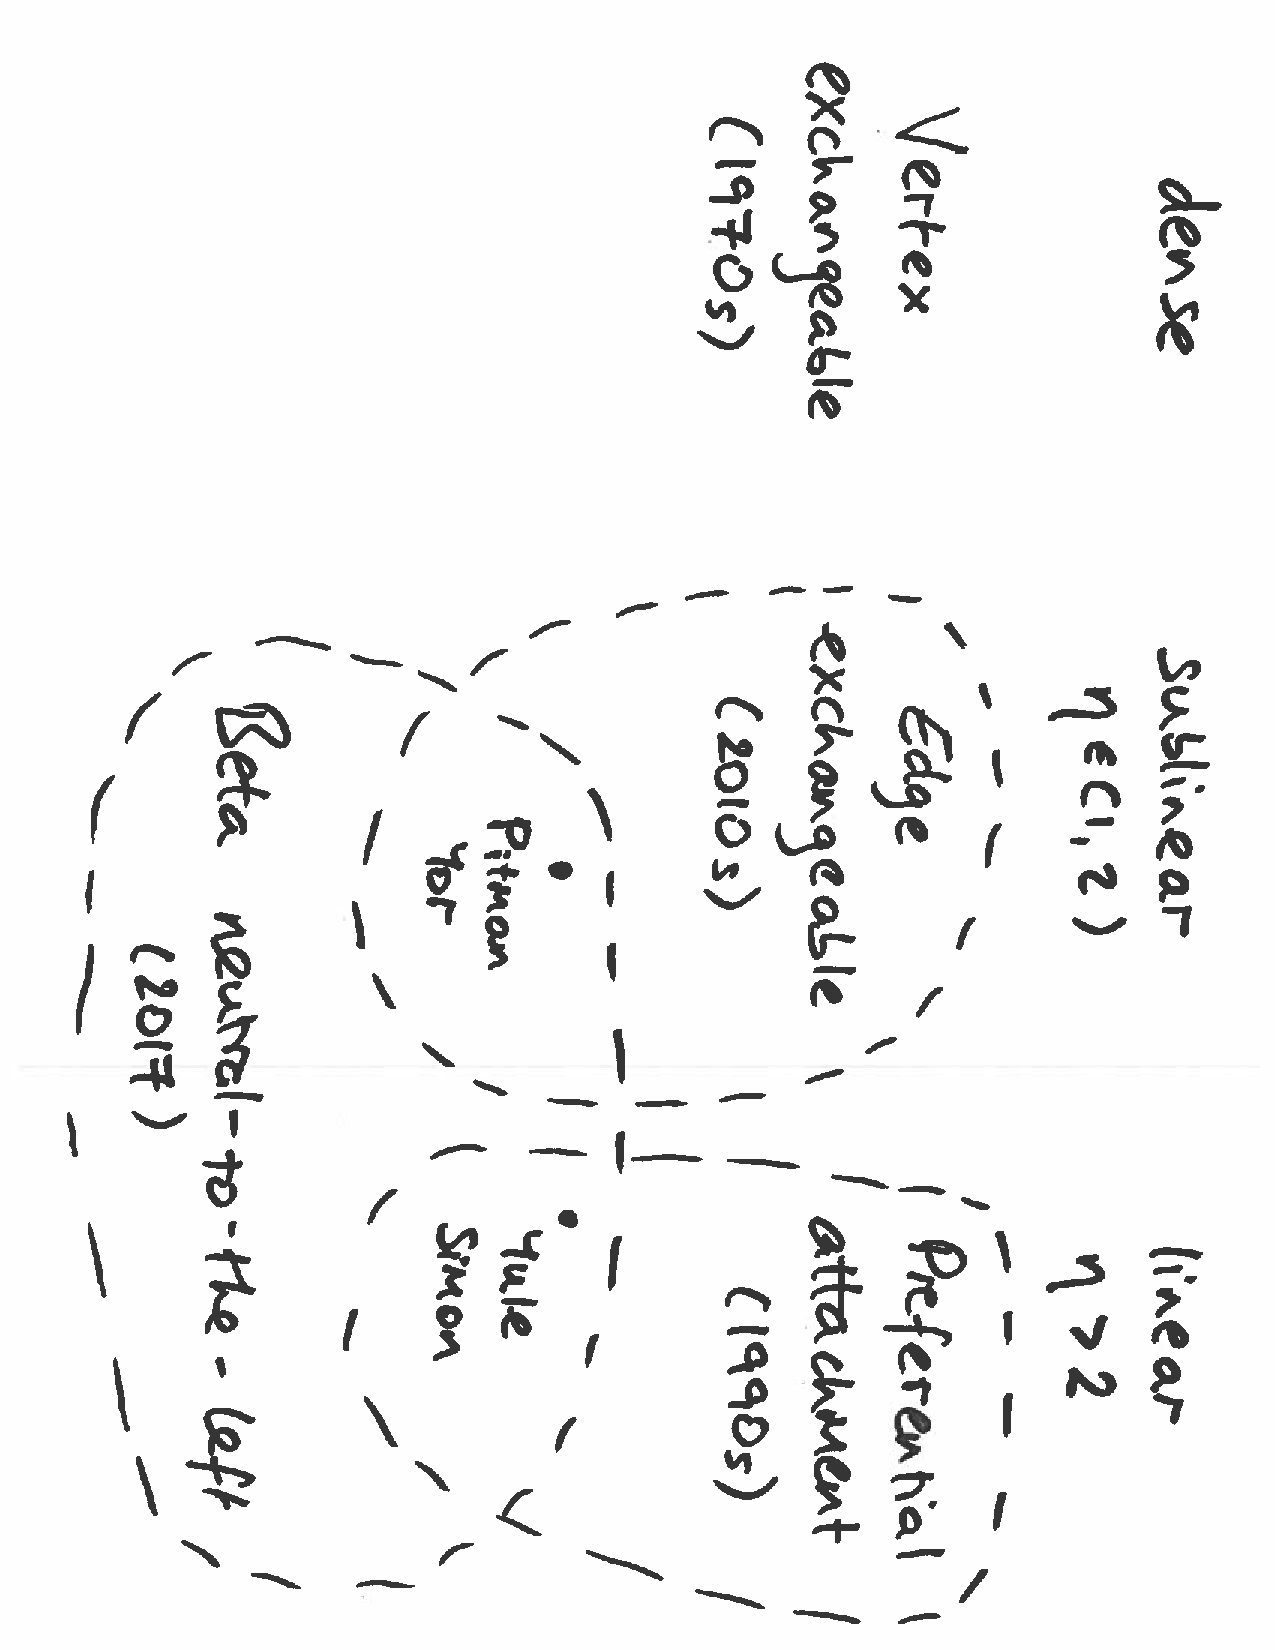
\includegraphics[angle=90,origin=c,scale=0.4]{fig/models}
\end{frame}

\begin{frame}
	\frametitle{Hierarchical representation of BNTL process}
	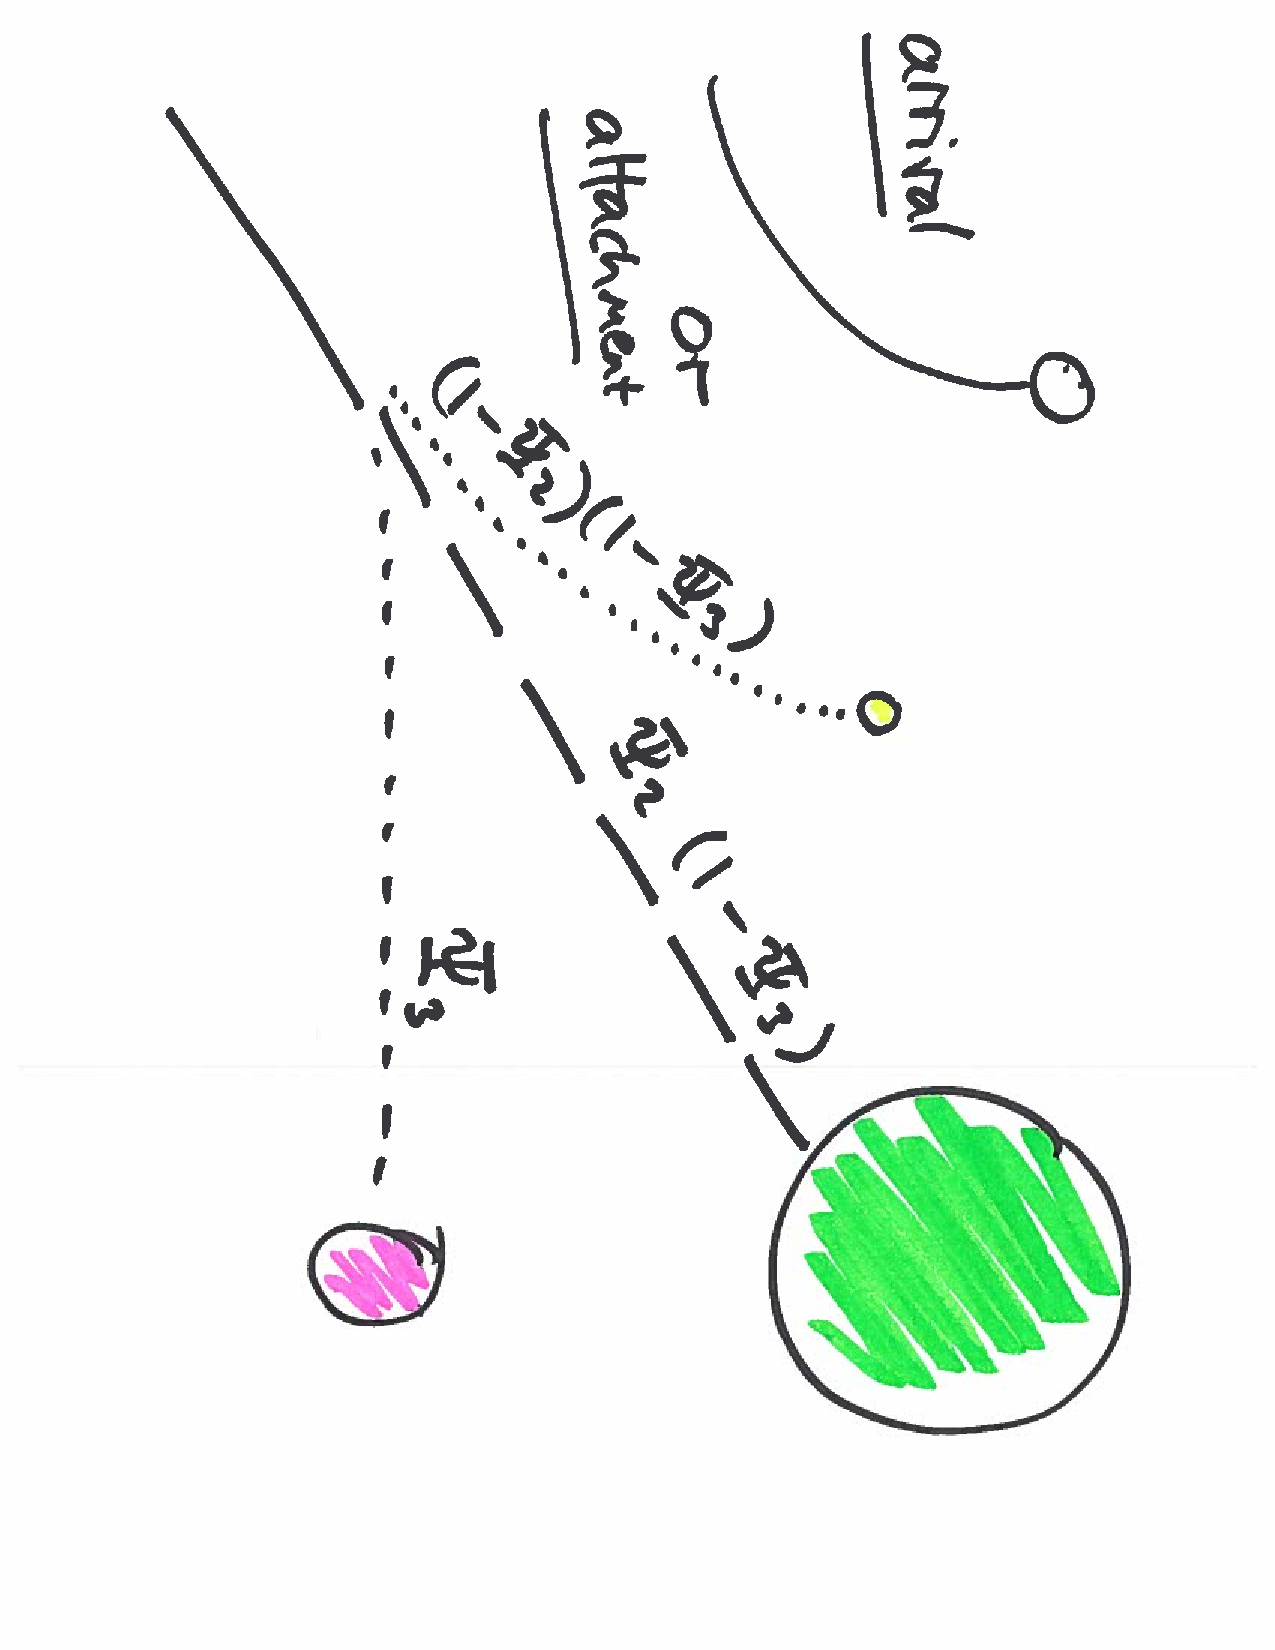
\includegraphics[angle=90,origin=c,scale=0.4]{fig/bntllatent}
\end{frame}

\begin{frame}
	\frametitle{Recursive scaling of BNTL latents}
	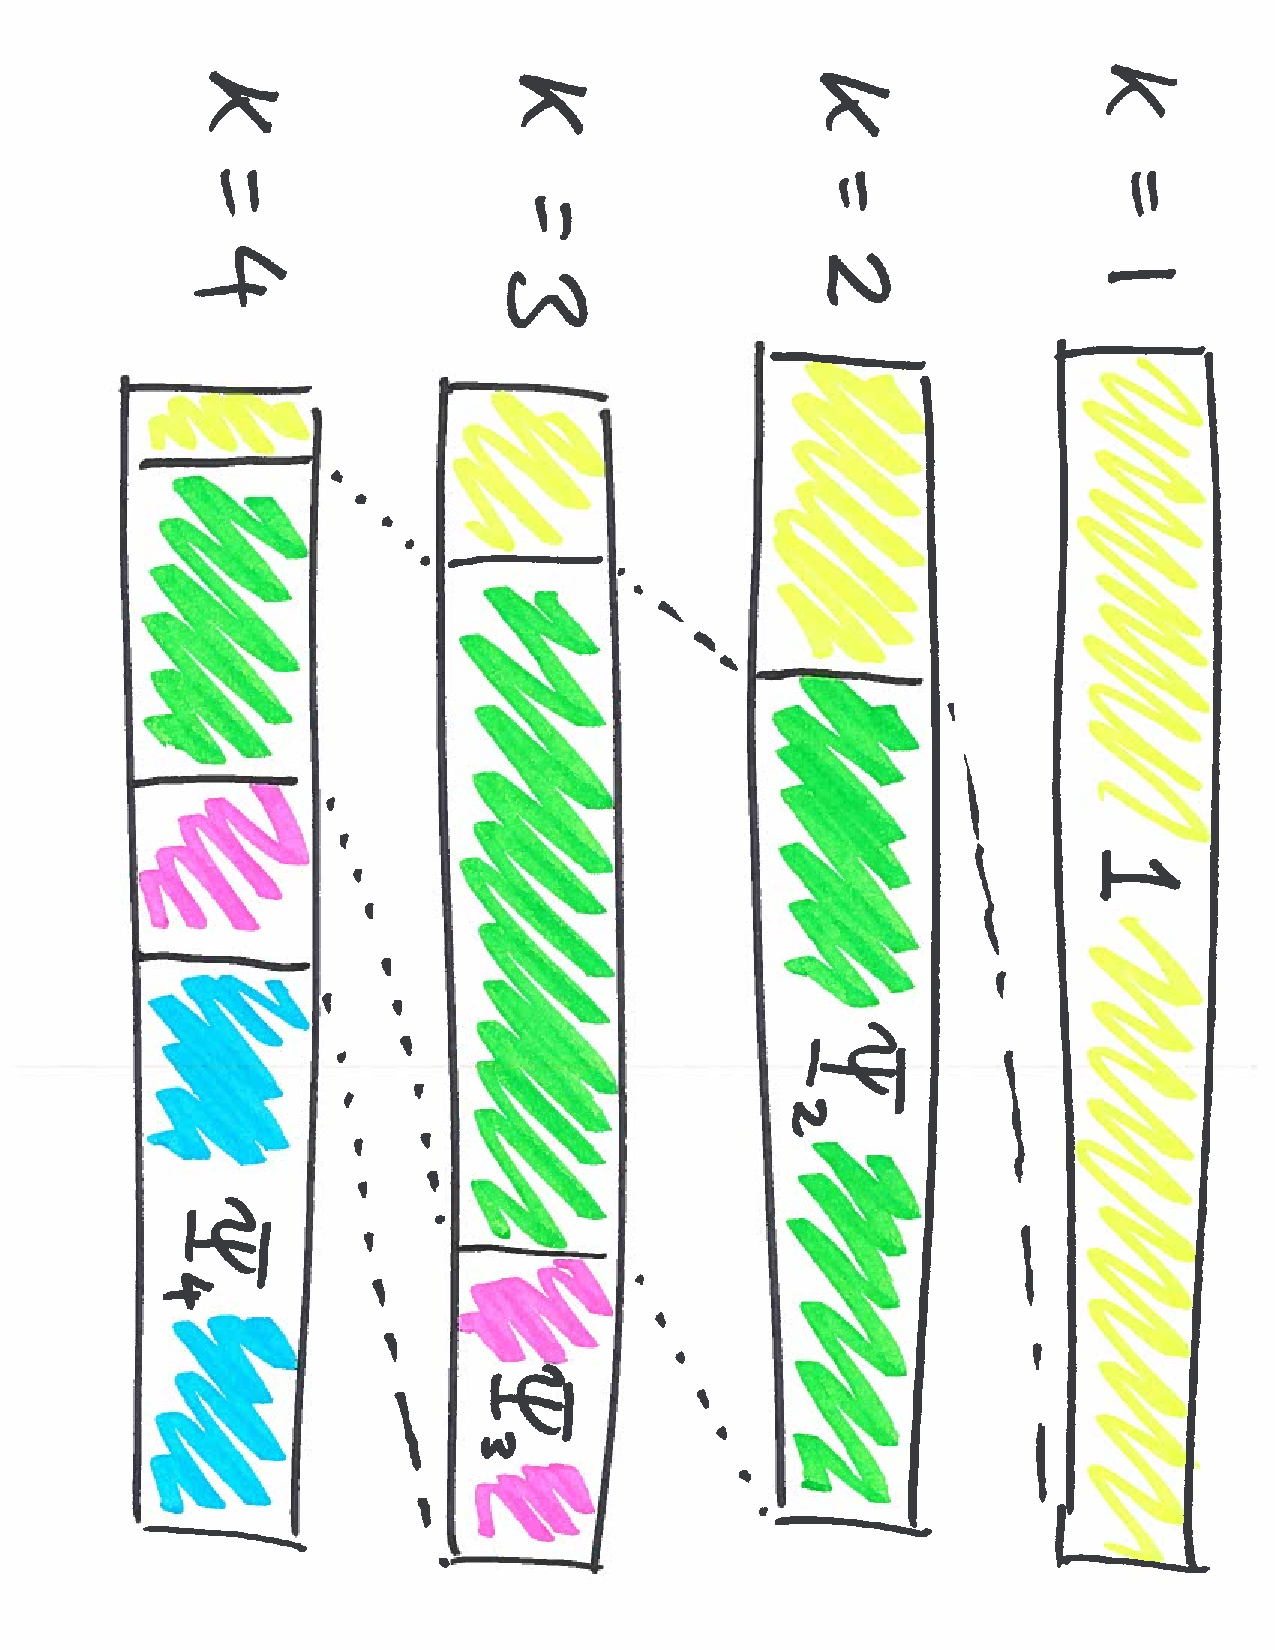
\includegraphics[angle=90,origin=c,scale=0.4]{fig/recursivescaling}
\end{frame}

\begin{frame}
	\frametitle{BNTL properties}
	\begin{itemize}
		\item Collapsed sampler
		\item Latent representation \textbf{not} from de Finetti
	\end{itemize}
\end{frame}


\section{Sampling and inference}
\begin{frame}
	\frametitle{Sampling and inference}
	Three observation cases
	\begin{itemize}
		\item Entire history
		\item Vertex order
		\item Snapshot
	\end{itemize}
\end{frame}

\begin{frame}
	\frametitle{Entire history}
	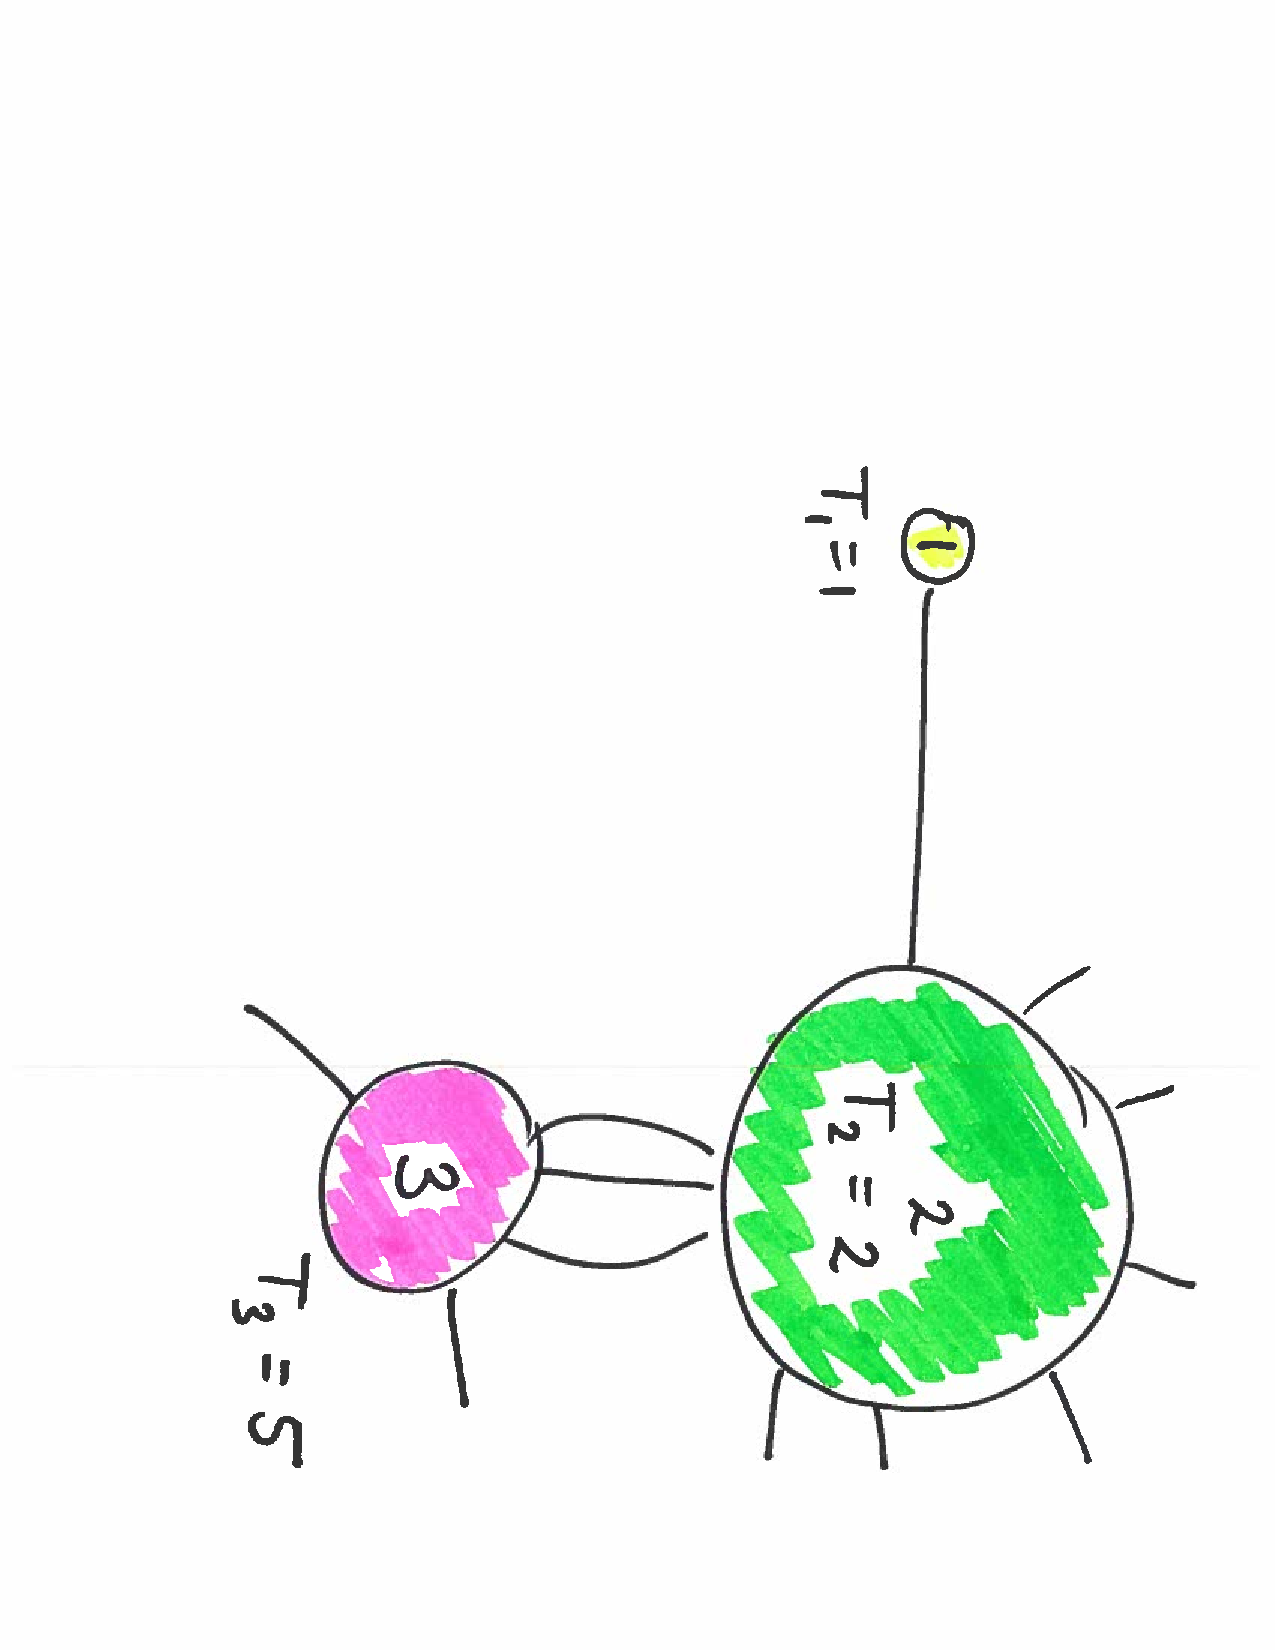
\includegraphics[angle=90,origin=c,scale=0.4]{fig/observeall}
\end{frame}

\begin{frame}
	\frametitle{Vertex order}
	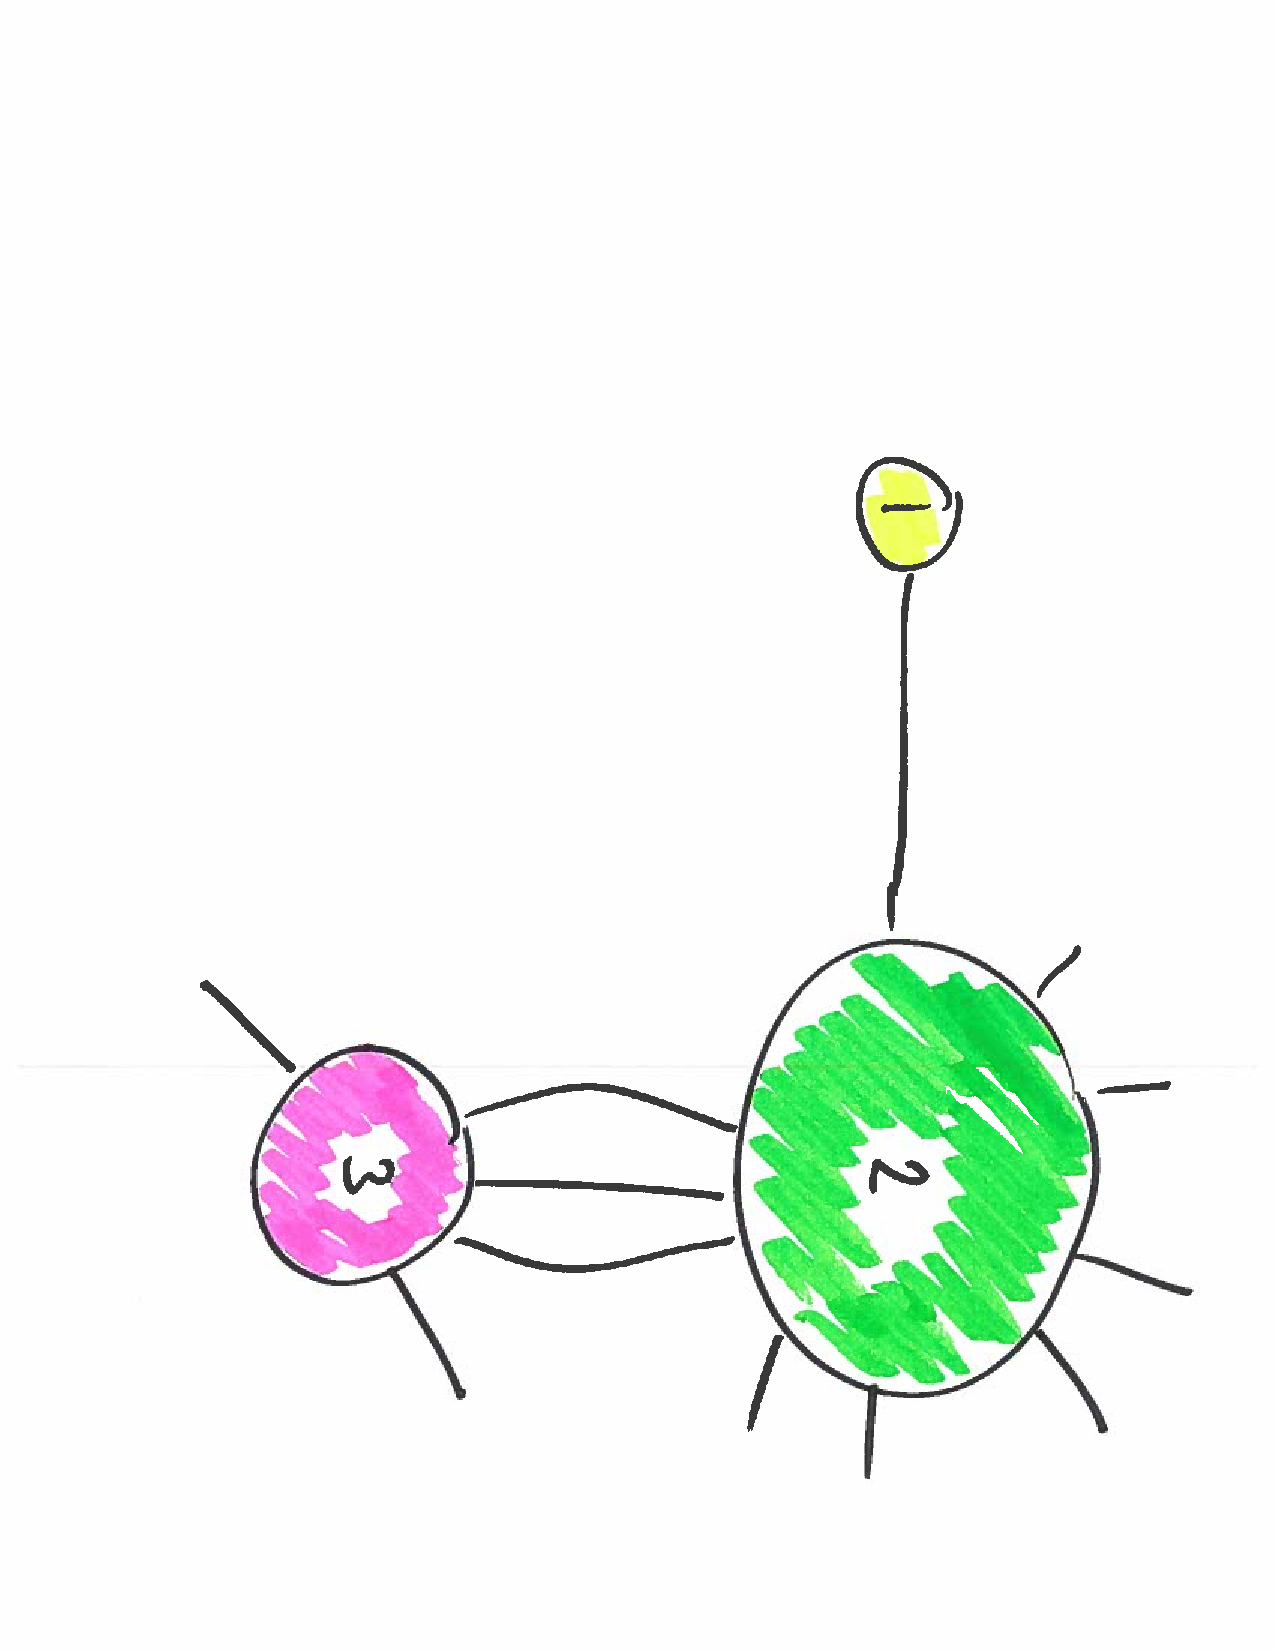
\includegraphics[angle=90,origin=c,scale=0.4]{fig/observeorder}
\end{frame}

\begin{frame}
	\frametitle{Snapshot}
	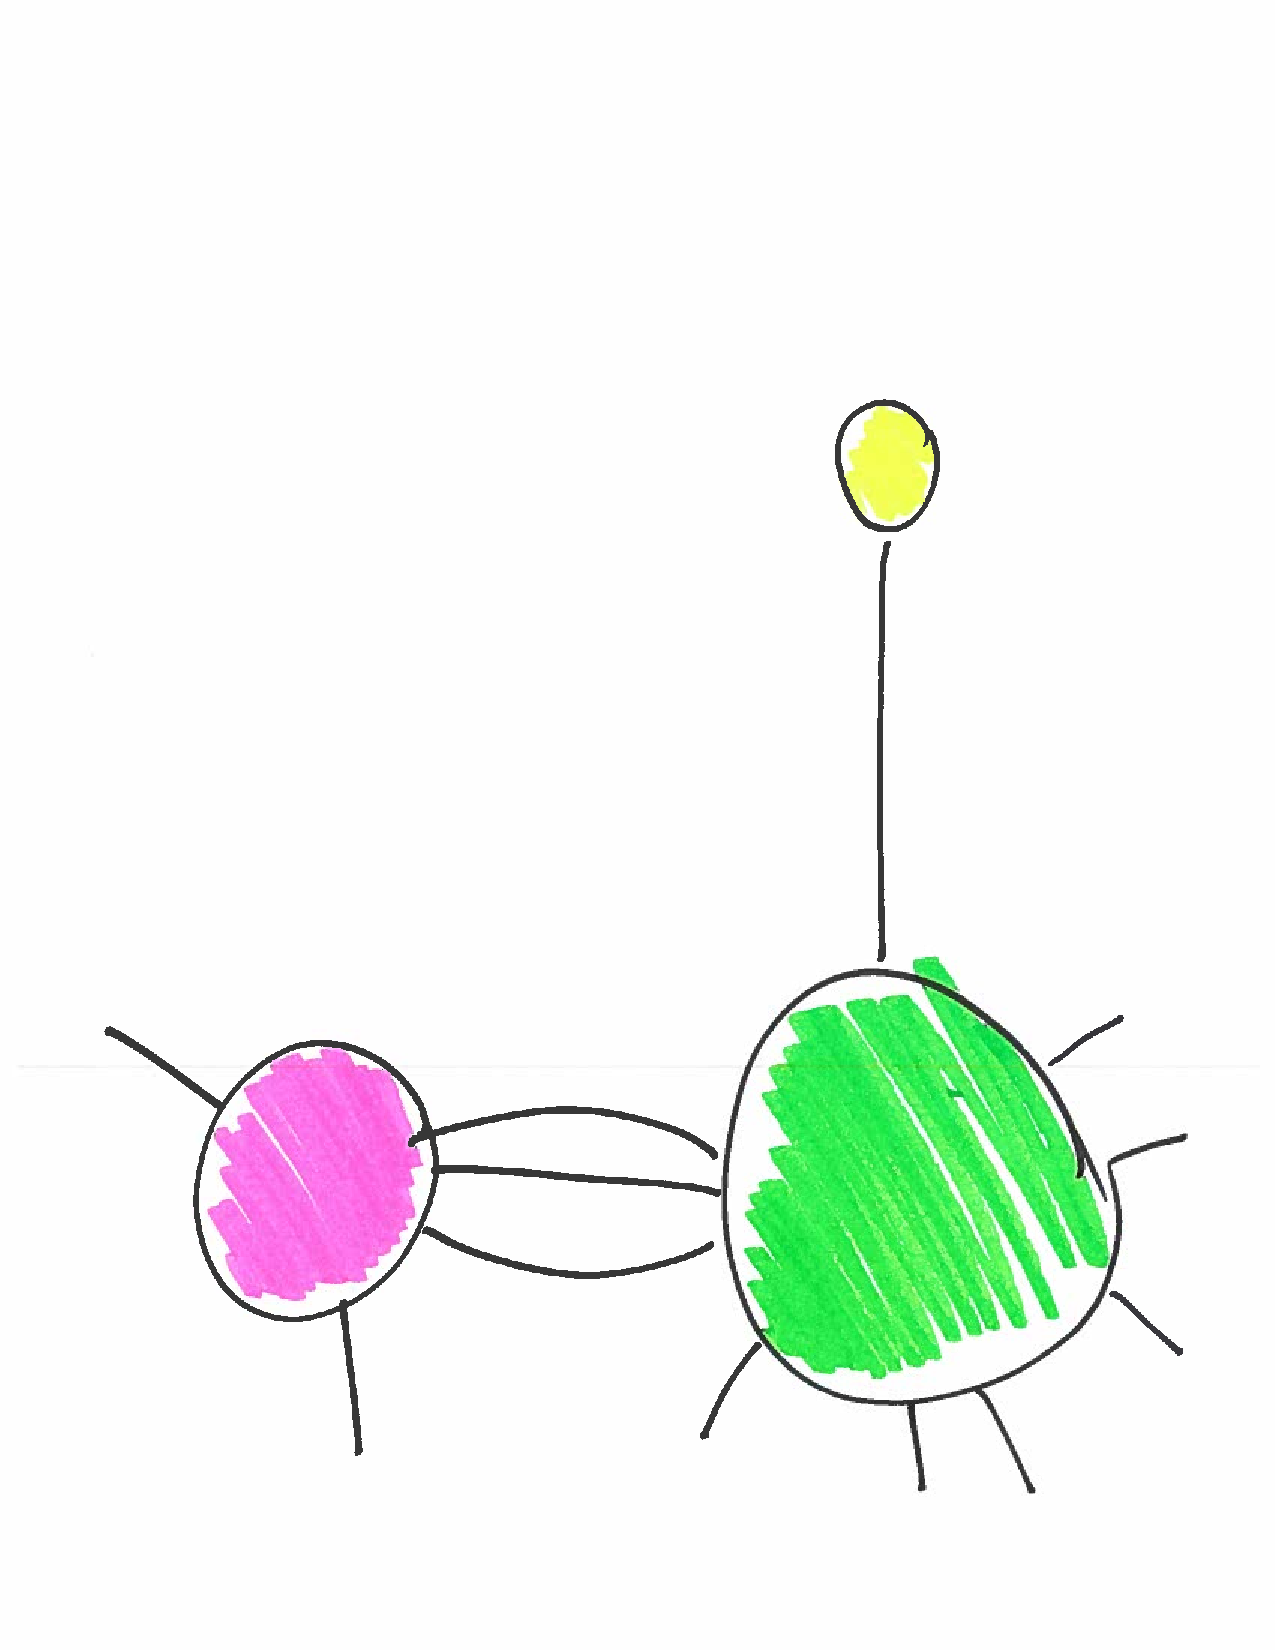
\includegraphics[angle=90,origin=c,scale=0.4]{fig/observesnap}
\end{frame}

\begin{frame}
	\frametitle{Observation cases}
	\begin{center}
		\begin{tabular}{ll}
			\textbf{Observation} & \textbf{Unobserved variables} \\
			\hline
			Entire history & $\alpha,\phi,\bfPsi_{K_n}$ \\
			Vertex order & $\alpha,\phi,\bfPsi_{K_n}, \bfT_{K_n}$ \\
			Snapshot & $\alpha,\phi,\bfPsi_{K_n},\bfT_{K_n},\sigma [K_n]$
		\end{tabular}
	\end{center}
\end{frame}

\begin{frame}
	\frametitle{Sampling $\bfPsi$}
	Beta prior on $\Psi_j$, plus recursive scaling --
	\begin{equation*}
	\Psi_j \mid \bfee_n, \bfPsi_{\setminus j} \sim \text{Beta}(d_{j,n} - \alpha, \bar{d}_{j-1,n} - (j-1)\alpha) \;,
	\end{equation*}
	
	\begin{itemize}
		\item For fixed $\alpha$, we have our posterior
		\item Learning other variables, we have a Gibbs update
	\end{itemize}
\end{frame}

\begin{frame}
	\frametitle{Sampling $\alpha, \phi$}
	\begin{itemize}
		\item For $\alpha$, one-dimensional unnormalized density
		\item For $\phi$, depends on family. Our experiments used conjugacy or slice sampling.
	\end{itemize}

\end{frame}

\begin{frame}
	\frametitle{Sampling $\bfT$}
	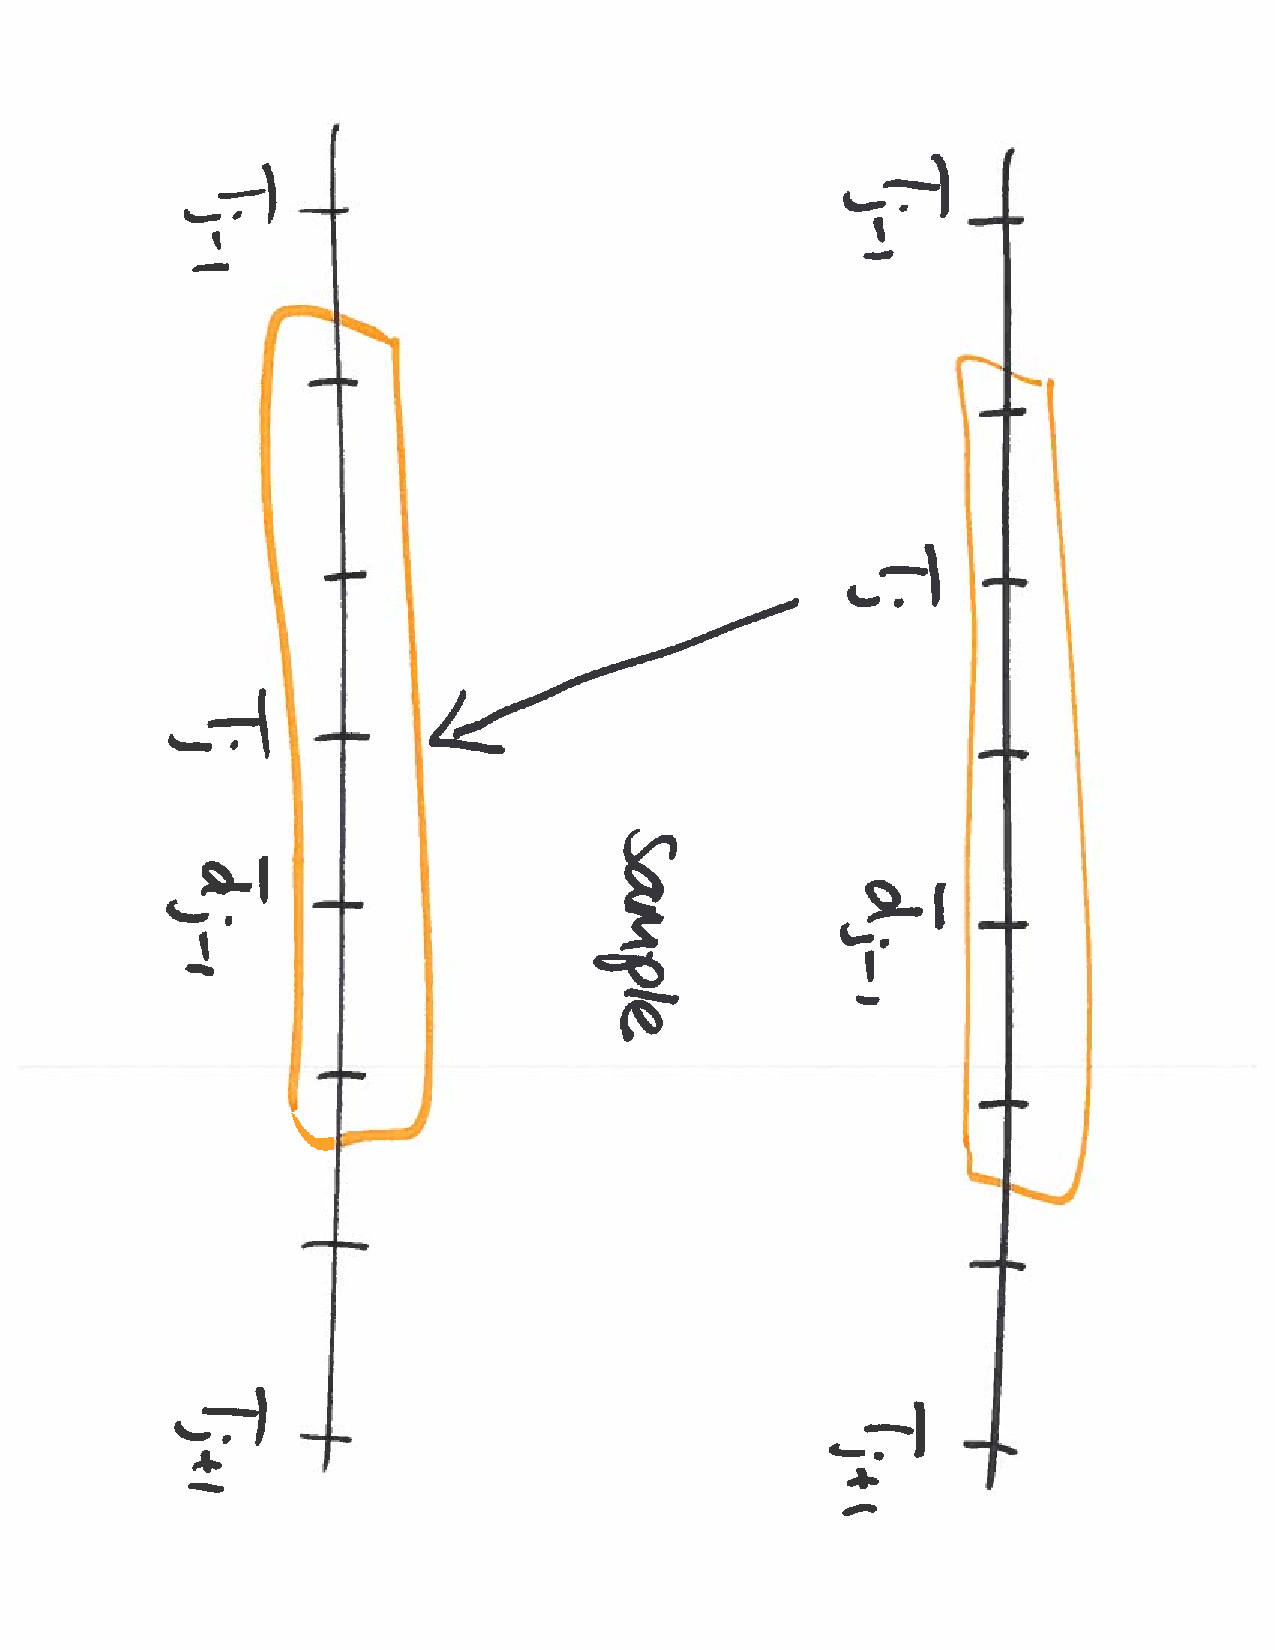
\includegraphics[angle=90,origin=c,scale=0.4]{fig/tsampling}
	
\end{frame}

\begin{frame}
	\frametitle{Sampling $\sigma[K_n]$}\

	\begin{itemize} 
	\item Use Metropolis-Hastings with swap proposal $\sigma_j \leftrightarrow \sigma_{j+1}$
	\end{itemize}
\end{frame}

\begin{frame}
	\frametitle{Point estimation}
	\begin{itemize}
		\item MLE/MAP estimation for $\alpha, \phi$ by optimizing unnormalized density
	\end{itemize}
\end{frame}

\section{Experiments}
\begin{frame}
	\frametitle{Experiments}
	\begin{itemize}
		\item Synthetic data -- parameter recovery
		\item Scaling in $n$
		\item Point estimation with massive graphs
	\end{itemize}
\end{frame}

\begin{frame}
	\frametitle{Synthetic data}
	\begin{itemize}
		\item Simulate 500 edges from the prior with fixed $\alpha$ 
		\item Arrivals either $\PYP$ or $\Geom$
		\item Observe final snapshot of the graph only
	\end{itemize}
\end{frame}

\begin{frame}
	\frametitle{Gibbs sampler results}
	\begin{table}[h]
		%  \caption{Results of Gibbs sampling experiments on synthetic data $(\alpha^* = 0.75)$. The top four rows show results from each of four different BNTL models fit to a synthetic graph with 500 edges generated by the coupled $\PYP$ BNTL model; the bottom four rows show the same BNTL models fit to a synthetic graph with $\Geom(0.25)$-distributed interarrivals.}
		\label{tab:ess}
		\vspace*{-0.75\baselineskip}
		\begin{center}
			\resizebox{1.0\textwidth}{!}{
				\begin{tabular}{lllll}
					Gen. arrival distn. & Inference model & $|\hat{\alpha} - \alpha^*|$ & Pred. log-lik.  \\
					\hline
					$\PYP(1.0,0.75)$ &  $(\tau,\PYP(\theta,\tau))$ &  \textbf{0.046 $\pm$ 0.002}   & -\textbf{2637.0 $\pm$ 0.1}  \\ 
					
					$\PYP(1.0,0.75)$  &  $(\alpha,\Geom(\beta))$  &  {0.049 $\pm$ 0.004} & -2660.5 $\pm$ 0.7  \\ 
					\hline
					
					$\Geom(0.25)$ & $(\tau,\PYP(\theta,\tau))$ &  0.086 $\pm$ 0.002   & -2386.8 $\pm$ 0.1  \\  
					
					$\Geom(0.25)$ & $(\alpha,\Geom(\beta))$ &  \textbf{0.043 $\pm$ 0.003}  & -\textbf{2382.6 $\pm$ 0.2}  \\ 
					
					\end{tabular}
					}
				\end{center}
			\end{table}
			
% where $\mathbf{S} := \frac{1}{K_n - 1} \sum_{j>1} (\bar{d}_{j-1} - T_j)$
\end{frame}

\begin{frame}
	\frametitle{Scalability of Gibbs sampler}
	\begin{itemize}
		\item Do we learn from all data?
		\item How does performance scale?
	\end{itemize}
	\pause
	
	\begin{table}[t]
		\label{tab:ess:scale:n}
		\vspace*{-0.25\baselineskip}
		\begin{center}
			%  \resizebox{0.6\textwidth}{!}{
			\begin{tabular}{l  ll}
				& $n=200$ &  $n=20000$ \\ 
				\hline
				$|\hat{\alpha} - \alpha^*|$ & 0.12 $\pm$ 0.01 &  0.01 $\pm$ 0.00 \\ 
				
				$|\hat{\beta} - \beta^*|$ &  0.02 $\pm$ 0.00  &    0.00 $\pm$ 0.00  \\ 
				
				ESS &  0.90 $\pm$ 0.04  &   0.75 $\pm$ 0.08  \\  
				
				Runtime (s) &  21 $\pm$ 0   &  2267 $\pm$ 2  \\ 
				
			\end{tabular}
			%}
		\end{center}
	\end{table}
	\begin{itemize}
		\item Most expensive Gibss update is for $\bfT$
	\end{itemize}
\end{frame}

\begin{frame}
	\frametitle{MLEs for SNAP datasets}
	Fitted point estimates
	\begin{table}[!ht]
		\begin{center}
			\color{lightgray}{
				\resizebox{1.05\textwidth}{!}{
					\begin{tabular}{llll | lllllll}
						\multirow{2}{*}{Dataset} & \multicolumn{3}{c}{\color{black}{Coupled $\PYP(\theta,\alpha)$}}  & &  \multicolumn{2}{c}{\color{black}{Uncoupled $\PYP(\theta,\tau)$}} &  & \multicolumn{3}{c}{\color{black}{$\Geom(\geom)$}}                             \\
						\cline{2-4} \cline{6-7} \cline{9-11}
						& \color{black}{$(\hat{\theta},\hat{\alpha})$} & $\hat{\eta}$           & \color{black}{Pred. l-l.}            & \color{black}{$\hat{\alpha}$}    & \color{black}{$(\hat{\theta},\hat{\tau})$} & \color{black}{Pred. l-l.}     &     & \color{black}{$\hat{\beta}$}  & $\hat{\eta}$   & \color{black}{Pred. l-l.}                             \\
						\hline
						\color{black}{Ask Ubuntu}  & (18080, 0.25) & 1.25   & -3.707e6              & -2.54            & (-0.99, 0.99)    & -3.678e6  &   &  0.083 & 2.32    & \textbf{-3.678e6}                         \\
						\color{black}{UCI social network} & (320.4, 4.4e-11) & --   & -1.600e5            & -4.98             & (5.50, 0.52)     & \textbf{-1.595e6}   &  & 0.016  & 2.10  & -1.596e5                    \\
						\color{black}{EU email}   & (113.6, 2.5e-14)  & --    & \textbf{-8.06e5}              & -1.86              & (113.6, 9.2e-10)      & \textbf{-8.06e5}  &   & 0.001  & 2.00   & -8.07e5                     \\
						\color{black}{Math Overflow} & (2575, 0.15) & 1.15  & -1.685e6              & -6.62           & (-0.97, 0.997)    & -1.670e6 &    & 0.025  & 2.19   & \textbf{-1.670e6}                \\
						\color{black}{Stack Overflow} & (297600, 0.11) & 1.11 & -3.358e8             & -8.94            & (-1.0, 1.0)      &  -3.333e8  &    &  0.020  & 2.21   & \textbf{-3.333e8}                 \\
						\color{black}{Super User}  & (20640, 0.24) & 1.24  & -5.855e6            & -4.19          & (-0.996, 1.0)      &  \textbf{-5.775e6}   &  & 0.067 & 2.37    & -5.775e6              \\
						\color{black}{Wikipedia talk pages}  & (14870, 0.54) & 1.54  & -3.074e7          & -0.25            & (-1.0, 1.0)   & \textbf{-3.066e7}  &   & 0.073  & 2.10   & -3.066e7                   
					\end{tabular}
				}}
			\end{center}
			\vspace*{-\baselineskip}
		\end{table}
	\end{frame}

\begin{frame}
	\frametitle{MLEs for SNAP datasets}
	$\PYP$ parameter estimates vary coupled and uncoupled
	\begin{table}[!ht]
		\begin{center}
			\color{lightgray}{
			\resizebox{1.05\textwidth}{!}{
				\begin{tabular}{llll | lllllll}
					\multirow{2}{*}{Dataset} & \multicolumn{3}{c}{\color{black}{Coupled $\PYP(\theta,\alpha)$}}  & &  \multicolumn{2}{c}{\color{black}{Uncoupled $\PYP(\theta,\tau)$}} &  & \multicolumn{3}{c}{$\Geom(\geom)$}                             \\
					\cline{2-4} \cline{6-7} \cline{9-11}
					& \color{black}{$(\hat{\theta},\hat{\alpha})$} & $\hat{\eta}$           & Pred. l-l.            & \color{black}{$\hat{\alpha}$}    & \color{black}{$(\hat{\theta},\hat{\tau})$} & Pred. l-l.     &     & $\hat{\beta}$  & $\hat{\eta}$   & Pred. l-l.                             \\
					\hline
					Ask Ubuntu  & \color{black}{(18080, 0.25)} & 1.25   & -3.707e6              & \color{black}{-2.54}            & \color{black}{(-0.99, 0.99)}    & -3.678e6  &   &  0.083 & 2.32    & \textbf{-3.678e6}                         \\
					UCI social network & (320.4, 4.4e-11) & --   & -1.600e5            & -4.98             & (5.50, 0.52)     & \textbf{-1.595e6}   &  & 0.016  & 2.10  & -1.596e5                    \\
					EU email   & (113.6, 2.5e-14)  & --    & \textbf{-8.06e5}              & -1.86              & (113.6, 9.2e-10)      & \textbf{-8.06e5}  &   & 0.001  & 2.00   & -8.07e5                     \\
					Math Overflow & (2575, 0.15) & 1.15  & -1.685e6              & -6.62           & (-0.97, 0.997)    & -1.670e6 &    & 0.025  & 2.19   & \textbf{-1.670e6}                \\
					Stack Overflow & \color{black}{(297600, 0.11)} & 1.11 & -3.358e8             & \color{black}{-8.94}            & \color{black}{(-1.0, 1.0)}      &  -3.333e8  &    &  0.020  & 2.21   & \textbf{-3.333e8}                 \\
					Super User  & (20640, 0.24) & 1.24  & -5.855e6            & -4.19          & (-0.996, 1.0)      &  \textbf{-5.775e6}   &  & 0.067 & 2.37    & -5.775e6              \\
					Wikipedia talk pages  & (14870, 0.54) & 1.54  & -3.074e7          & -0.25            & (-1.0, 1.0)   & \textbf{-3.066e7}  &   & 0.073  & 2.10   & -3.066e7                   
				\end{tabular}
			}}
		\end{center}
		\vspace*{-\baselineskip}
	\end{table}
\end{frame}

\begin{frame}
	\frametitle{MLEs for SNAP datasets}
	Edge exchangeable models likely misspecified 
	\begin{table}[!ht]
		\begin{center}
			\color{lightgray}{
				\resizebox{1.05\textwidth}{!}{
					\begin{tabular}{llll | lllllll}
						\multirow{2}{*}{Dataset} & \multicolumn{3}{c}{Coupled $\PYP(\theta,\alpha)$}  & &  \multicolumn{2}{c}{Uncoupled $\PYP(\theta,\tau)$} &  & \multicolumn{3}{c}{\color{black}{$\Geom(\geom)$}}                             \\
						\cline{2-4} \cline{6-7} \cline{9-11}
						& $(\hat{\theta},\hat{\alpha})$ & $\hat{\eta}$           & Pred. l-l.            & $\hat{\alpha}$    & $(\hat{\theta},\hat{\tau})$ & Pred. l-l.     &     & $\hat{\beta}$  & \color{black}{$\hat{\eta}$}   & Pred. l-l.                             \\
						\hline
						\color{black}{Ask Ubuntu}  & (18080, 0.25) & 1.25   & -3.707e6              & -2.54            & (-0.99, 0.99)    & -3.678e6  &   &  0.083 & \color{black}{2.32}    & \textbf{-3.678e6}                         \\
						UCI social network & (320.4, 4.4e-11) & --   & -1.600e5            & -4.98             & (5.50, 0.52)     & \textbf{-1.595e6}   &  & 0.016  & 2.10  & -1.596e5                    \\
						EU email   & (113.6, 2.5e-14)  & --    & \textbf{-8.06e5}              & -1.86              & (113.6, 9.2e-10)      & \textbf{-8.06e5}  &   & 0.001  & 2.00   & -8.07e5                     \\
						Math Overflow & (2575, 0.15) & 1.15  & -1.685e6              & -6.62           & (-0.97, 0.997)    & -1.670e6 &    & 0.025  & 2.19   & \textbf{-1.670e6}                \\
						\color{black}{Stack Overflow} & (297600, 0.11) & 1.11 & -3.358e8             & -8.94            & (-1.0, 1.0)      &  -3.333e8  &    &  0.020  & \color{black}{2.21}   & \textbf{-3.333e8}                 \\
						Super User  & (20640, 0.24) & 1.24  & -5.855e6            & -4.19          & (-0.996, 1.0)      &  \textbf{-5.775e6}   &  & 0.067 & 2.37    & -5.775e6              \\
						Wikipedia talk pages  & (14870, 0.54) & 1.54  & -3.074e7          & -0.25            & (-1.0, 1.0)   & \textbf{-3.066e7}  &   & 0.073  & 2.10   & -3.066e7                   
					\end{tabular}
				}}
			\end{center}
			\vspace*{-\baselineskip}
		\end{table}
	\end{frame}
	
\begin{frame}
	\frametitle{MLEs for SNAP datasets}
	Though better than $\Geom$ for some datasets
	\begin{table}[!ht]
		\begin{center}
			\color{lightgray}{
				\resizebox{1.05\textwidth}{!}{
					\begin{tabular}{llll | lllllll}
						\multirow{2}{*}{Dataset} & \multicolumn{3}{c}{Coupled $\PYP(\theta,\alpha)$}  & &  \multicolumn{2}{c}{Uncoupled $\PYP(\theta,\tau)$} &  & \multicolumn{3}{c}{$\Geom(\geom)$}                             \\
						\cline{2-4} \cline{6-7} \cline{9-11}
						& $(\hat{\theta},\hat{\alpha})$ & $\hat{\eta}$           & Pred. l-l.            & $\hat{\alpha}$    & $(\hat{\theta},\hat{\tau})$ & Pred. l-l.     &     & $\hat{\beta}$  & $\hat{\eta}$   & Pred. l-l.                             \\
						\hline
						Ask Ubuntu  & (18080, 0.25) & 1.25   & -3.707e6              & -2.54            & (-0.99, 0.99)    & -3.678e6  &   &  0.083 & 2.32    & \textbf{-3.678e6}                         \\
						UCI social network & (320.4, 4.4e-11) & --   & -1.600e5            & -4.98             & (5.50, 0.52)     & \textbf{-1.595e6}   &  & 0.016  & 2.10  & -1.596e5                    \\
						\color{black}{EU email}   & \color{black}{(113.6, 2.5e-14)}  & --    & \color{black}{\textbf{-8.06e5}}              & \color{black}{-1.86}              & \color{black}{(113.6, 9.2e-10)}      & \color{black}{\textbf{-8.06e5}}  &   & \color{black}{0.001}  & \color{black}{2.00}   & \color{black}{-8.07e5}                     \\
						Math Overflow & (2575, 0.15) & 1.15  & -1.685e6              & -6.62           & (-0.97, 0.997)    & -1.670e6 &    & 0.025  & 2.19   & \textbf{-1.670e6}                \\
						Stack Overflow & (297600, 0.11) & 1.11 & -3.358e8             & -8.94            & (-1.0, 1.0)      &  -3.333e8  &    &  0.020  & 2.21   & \textbf{-3.333e8}                 \\
						Super User  & (20640, 0.24) & 1.24  & -5.855e6            & -4.19          & (-0.996, 1.0)      &  \textbf{-5.775e6}   &  & 0.067 & 2.37    & -5.775e6              \\
						Wikipedia talk pages  & (14870, 0.54) & 1.54  & -3.074e7          & -0.25            & (-1.0, 1.0)   & \textbf{-3.066e7}  &   & 0.073  & 2.10   & -3.066e7                   
					\end{tabular}
				}}
			\end{center}
			\vspace*{-\baselineskip}
		\end{table}
	\end{frame}
	
%\begin{frame}
%	\frametitle{MLEs for SNAP datasets}
%	Though not for all datasets
%	\begin{table}[!ht]
%		\begin{center}
%			\color{lightgray}{
%				\resizebox{1.05\textwidth}{!}{
%					\begin{tabular}{llll | lllllll}
%						\multirow{2}{*}{Dataset} & \multicolumn{3}{c}{Coupled $\PYP(\theta,\alpha)$}  & &  \multicolumn{2}{c}{Uncoupled $\PYP(\theta,\tau)$} &  & \multicolumn{3}{c}{$\Geom(\geom)$}                             \\
%						\cline{2-4} \cline{6-7} \cline{9-11}
%						& $(\hat{\theta},\hat{\alpha})$ & $\hat{\eta}$           & Pred. l-l.            & $\hat{\alpha}$    & $(\hat{\theta},\hat{\tau})$ & Pred. l-l.     &     & $\hat{\beta}$  & $\hat{\eta}$   & Pred. l-l.                             \\
%						\hline
%						Ask Ubuntu  & (18080, 0.25) & 1.25   & -3.707e6              & -2.54            & (-0.99, 0.99)    & -3.678e6  &   &  0.083 & 2.32    & \textbf{-3.678e6}                         \\
%						UCI social network & (320.4, 4.4e-11) & --   & -1.600e5            & -4.98             & (5.50, 0.52)     & \textbf{-1.595e6}   &  & 0.016  & 2.10  & -1.596e5                    \\
%						EU email   & (113.6, 2.5e-14)  & --    & \textbf{-8.06e5}              & -1.86              & (113.6, 9.2e-10)      & \textbf{-8.06e5}  &   & 0.001  & 2.00   & -8.07e5                     \\
%						Math Overflow & (2575, 0.15) & 1.15  & -1.685e6              & -6.62           & (-0.97, 0.997)    & -1.670e6 &    & 0.025  & 2.19   & \textbf{-1.670e6}                \\
%						Stack Overflow & (297600, 0.11) & 1.11 & -3.358e8             & -8.94            & (-1.0, 1.0)      &  -3.333e8  &    &  0.020  & 2.21   & \textbf{-3.333e8}                 \\
%						Super User  & (20640, 0.24) & 1.24  & -5.855e6            & -4.19          & (-0.996, 1.0)      &  \textbf{-5.775e6}   &  & 0.067 & 2.37    & -5.775e6              \\
%						Wikipedia talk pages  & (14870, 0.54) & 1.54  & -3.074e7          & -0.25            & (-1.0, 1.0)   & \textbf{-3.066e7}  &   & 0.073  & 2.10   & -3.066e7                   
%					\end{tabular}
%				}}
%			\end{center}
%			\vspace*{-\baselineskip}
%		\end{table}
%	\end{frame}

\begin{frame}
	\frametitle{Conclusion}
	\begin{itemize}
		\item BNTL models are \textit{flexible}
		\item BNTL models are \textit{tractable}
	\end{itemize}
\end{frame}

\begin{frame}
	\frametitle{Future work}
	\begin{itemize}
		\item Scalability of inference
		\begin{itemize}
			\item Metropolis-Hastings to update $\bfT$ altogether
			\item Variational inference for $\bfT$ \cite{linderman2017}
		\end{itemize}
		\item Recency-weighted preferential attachment
	\end{itemize}
\end{frame}

\begin{frame}
	\frametitle{References}
	\tiny{\bibliographystyle{unsrt}
	\bibliography{refs}}
\end{frame}

\end{document}
